\documentclass[numberedappendix]{emulateapj}
%\documentclass[iop]{emulateapj}
%apj gives the referee version/preprint2
%\usepackage[T1]{fontenc}
%\usepackage[utf8]{inputenc}
%\usepackage{graphicx}
%\usepackage{natbib}
\usepackage{amsmath}
\usepackage{amssymb}
%\usepackage{vmargin}
%\usepackage{pdfpages}
\usepackage{aas_macros}
\usepackage[normalem]{ulem}
\usepackage[usenames]{color}
\usepackage{bm}
\usepackage{cancel}
\definecolor{DarkGreen}{rgb}{0.64,0.80,0.35}
\newcommand\ALc[1]{{\color{red} \bf #1}} %Astrid
\newcommand\Ac[1]{{\color{green} \bf #1}} %% Avery
\newcommand\Pc[1]{{\color{cyan} \bf #1}} %% Phil
\newcommand\Cc[1]{{\color{blue} \bf #1}} %% Christoph
\newcommand\Ec[1]{{\color{magenta} \bf #1}} %% Ewald

\DeclareMathAlphabet\mathbfcal{OMS}{cmsy}{b}{n}
\newcommand{\calR}{\ensuremath{\bm\hat{\mathbfcal{R}}}}
\newcommand{\magcalR}{\ensuremath{\hat{\mathcal{R}}}}

\SetSymbolFont{symbols}{bold}{OMS}{cmsy}{b}{n}
%
\DeclareSymbolFont{bmisymbols}{OML}{cmm}{b}{it}
\DeclareMathSymbol{\balpha}{0}{bmisymbols}{"0B}
\DeclareMathSymbol{\bbeta}{0}{bmisymbols}{"0C}
\DeclareMathSymbol{\bgamma}{0}{bmisymbols}{"0D}
\DeclareMathSymbol{\bdelta}{0}{bmisymbols}{"0E}
\DeclareMathSymbol{\bepsilon}{0}{bmisymbols}{"0F}
\DeclareMathSymbol{\bzeta}{0}{bmisymbols}{"10}
\DeclareMathSymbol{\boldeta}{0}{bmisymbols}{"11}
\DeclareMathSymbol{\btheta}{0}{bmisymbols}{"12}
\DeclareMathSymbol{\biota}{0}{bmisymbols}{"13}
\DeclareMathSymbol{\bkappa}{0}{bmisymbols}{"14}
\DeclareMathSymbol{\blambda}{0}{bmisymbols}{"15}
\DeclareMathSymbol{\bmu}{0}{bmisymbols}{"16}
\DeclareMathSymbol{\bnu}{0}{bmisymbols}{"17}
\DeclareMathSymbol{\bxi}{0}{bmisymbols}{"18}
\DeclareMathSymbol{\bpi}{0}{bmisymbols}{"19}
\DeclareMathSymbol{\brho}{0}{bmisymbols}{"1A}
\DeclareMathSymbol{\bsigma}{0}{bmisymbols}{"1B}
\DeclareMathSymbol{\btau}{0}{bmisymbols}{"1C}
\DeclareMathSymbol{\bupsilon}{0}{bmisymbols}{"1D}
\DeclareMathSymbol{\bphi}{0}{bmisymbols}{"1E}
\DeclareMathSymbol{\bchi}{0}{bmisymbols}{"1F}
\DeclareMathSymbol{\bpsi}{0}{bmisymbols}{"20}
\DeclareMathSymbol{\bomega}{0}{bmisymbols}{"21}
\DeclareMathSymbol{\bvarepsilon}{0}{bmisymbols}{"22}
\DeclareMathSymbol{\bvartheta}{0}{bmisymbols}{"23}
\DeclareMathSymbol{\bvarpi}{0}{bmisymbols}{"24}
\DeclareMathSymbol{\bvarrho}{0}{bmisymbols}{"25}
\DeclareMathSymbol{\bvarsigma}{0}{bmisymbols}{"26}
\DeclareMathSymbol{\bvarphi}{0}{bmisymbols}{"27}


\begin{document}
\title{Probing inhomogeneous blazar heating with the Ly$\alpha$ forest}
\author{Astrid Lamberts$^1$,  Ewald Puchwein$^2$ , Philip Chang$^3$ ,Christoph Pfrommer$^4$, Avery E. Broderick$^{5,6}$,  Mohamad Shalaby$^{5,6}$ and Alberto Rorai$^2$}
\affil{$^1$ Theoretical Astrophysics, California Institute of Technology, Pasadena, CA, 91125, USA}
\affil{$^2$ Institute of Astronomy and Kavli Institute for Cosmology, University of Cambridge, Madingley Road, Cambridge, CB3 0HA, UK}
\affil{$^3$ Department of Physics, University of Wisconsin-Milwaukee, 1900 East Kenwood Boulevard, Milwaukee WI 53211, USA}
\affil{$^4$ Heidelberg Institute for Theoretical Studies, Schloss-Wolfsbrunnenweg 35, D-69118 Heidelberg, Germany}
\affil{$^5$ Perimeter Institute for Theoretical Physics, 31 Caroline Street North, Waterloo, ON, N2L 2Y5, Canada}
\affil{$^6$ Department of Physics and Astronomy, University of Waterloo, 200 University Avenue West, Waterloo, ON, N2L 3G1, Canada}
\email{lamberts@caltech.edu}
\begin{abstract}

\end{abstract}
\keywords{}
\section{Introduction}

Even at the present day, the majority of the baryons resides in the intergalactic medium (IGM) rather than collapsed halos \ALc{cite} \citep{2012ApJ...759...23S}. The vast majority of ordinary matter is in a diffuse  state  between galaxies and is composed of gas around  and below the cosmic mean density $\Delta$\citep[see][for a recent review]{2016ARA&A..54..313M}. As the main reservoir for baryons,  its physical state sets the initial conditions for star formation. Due to its low density, the evolution of the IGM is mostly linear, closely follows the underlying dark matter and is directly influenced by fundamental cosmological parameters \citep{2013A&A...559A..85P,2013JCAP...04..026S,2015JCAP...11..011P}.  

Because of its linear nature, the IGM is an excellent calorimeter of energy injected by star formation and active galactic nuclei (AGN). More specifically, re-ionization of H and HeI around $z\simeq 10-6$ \citep{2006ARA&A..44..415F} and then HeII around $z\geqslant 3.5$ \Ec{[I think this is still controversial. May have finished at $z<3$.]} provide most of the heat input in the IGM \citep{2009ApJ...694..842M,2011ApJ...733L..24W}. Subsequently, the thermal evolution of the IGM is set by photoheating following recombinations and adiabatic cooling. Due to the Hubble expansion the IGM globally cools. The lowest density gas expands fastest and also receives least photoheating as there are fewer recombinations that allow subsequent photoionizations. Together this yields a tight temperature-density relation $T=T_0 \Delta ^{\gamma-1}$ for low density gas where $T_0$ is the temperature at the mean density and $\gamma$ asymptotically approaches $\simeq 1.6$  long after HeII reionization \citep{1997MNRAS.292...27H,2015MNRAS.450.4081P,2016MNRAS.456...47M}. 




During  and shortly after HeII re-ionization, the thermal state of the IGM is more complex.  Recent models of HeII re-ionisation, based on cosmological simulations including complete radiative transfer, indicate a patchy process yielding a broadening of the temperature-density distribution around and below mean density for $z\simeq 3$ \citep{2009ApJ...694..842M,2012MNRAS.423....7M,2013MNRAS.435.3169C}. \ALc{specify}.

 
The most dramatic impact on the low-density IGM could come from TeV-blazar heating \citep{2012ApJ...752...23C,2012MNRAS.423..149P,2015ApJ...811...19L}. This model is based on the electron/positron beams that result from the annihilation of TeV gamma-rays from blazars on the extragalactic background light. They can be subject to plasma instabilities, which efficiently redistribute their kinetic energy to the surrounding IGM \citep{2012ApJ...752...22B,2013ApJ...777...49S,2012ApJ...758..102S,2014ApJ...797..110C,2016ApJ...833..118C},  but see \citet{2013ApJ...770...54M,2014ApJ...787...49S}.  The resulting heating is only limited by the number of TeV-photons, which makes it a competitive heating source in the underdense regions, where photoheating is rendered impossible as the recombination time is larger than the Hubble time.  Assuming a uniform heating rate, it results in an inverted temperature-density distribution below the cosmic mean ($\gamma \leq 1$), with low density gas reaching  $10^5$K at $z=3$ and $\simeq 10^6$K in the present-day universe \citep{2012MNRAS.423..149P}.  



 %with potential impact on structure formation \citep{2012ApJ...752...24P}. 




Although uniform heating is a reasonable first order approximation, in \citet[hereafter Paper~I]{2015ApJ...811...19L} we showed that it is affected by the clustering of blazars. As a result, regions close to large overdense regions such as clusters or groups are receiving more heat than remote regions mostly surrounded by voids.  In our favoured model, where TeV blazars have the same bias as quasars, there are almost two orders of magnitude in temparature between the hottest and coldest gas between $z\simeq 2-3$. However, the bulk of the gas follows a temperature consistent with the uniform model. By the present day, all regions have been heated up and the uniform model provides a good description of the impact of blazar heating.

\ALc{should elaborate ob Ly a an beta?}
Determinig the thermal state of the IGM with observations is challenging, especially for the regions around or below the mean denstiy. The IGM is mostly observed through absorption lines within the spectra of distant quasars,  due to a tiny fraction of neutral hydrogen \citep{1971ApJ...164L..73L}. The so-called Ly$\alpha$ forest can be observed with ground-based facilities for $z\geq 1.7$  and with HST for $\leq 0.7$ \ALc{check and cite.}. A variety of statistics have been developed to analyse spectra from a wide range of instruments. However, deriving the physical parameters of the IGM from the different observables requires a careful calibration to cosmological simulations \citep[see e.g.][]{1997ApJ...489....7R,2000MNRAS.318..817S,2013MNRAS.436.1023B,2017MNRAS.464..897B}. The derivation of the temperature and density is also very sensitive to the assumed intensity and spectrum  of the ionising UV background, which is not firmly established, especially at low redshift \ALc{cite!}.
Because of the intrinsic observational challenges, numerical shortcomings and difficulty to establish the validity of the different statistics,  there is no observational consensus on the thermal state of the low-density IGM.

%Observational confirmation of blazar heating is a challenge, because it mostly affects low-density regions. The IGM is mostly observed through absorption lines within the spectra of distant quasars,  due to a tiny fraction of neutral hydrogen \citep{1971ApJ...164L..73L}. The so-called Ly$\alpha$ forest can be observed with ground-based facilities for $z\geq 1.7$ and a variety of statistics have been developed to analyse spectra from a wide range of instruments. However, deriving the physical parameters of the IGM from the different statistics requires a careful comparison with cosmological simulations \citep[see e.g.][]{1997ApJ...489....7R,2000MNRAS.318..817S,2013MNRAS.436.1023B,2017MNRAS.464..897B}. Because of the intrinsic observational challenges, numerical shortcomings and difficulty to establish the validity of the different statistics,  there is no observational consensus on the thermal state of the low-density IGM.
%and the difficulty to establish   %So far, there is no observational consensus on the thermal state of the IGM.

Different observational diagnostics suggest or disfavour the presence of blazar heating in the low density IGM. Based on the probability distribution function (PDF) of the transmitted Ly$\alpha$ flux, \citet{2007MNRAS.382.1657K,2008MNRAS.386.1131B,2009MNRAS.399L..39V,2012MNRAS.422.3019C} find that a flat or inverted  $T-\rho$ relation is in good agreement with the data. However, the flux PDF can be strongly affected by systematic errors in the continuum placement \citep{2012ApJ...753..136L} and sample variance \citep{2013MNRAS.428..540R}. Analysis of the curvature of the Ly$\alpha$ spectrum \citep{2011MNRAS.410.1096B,2014MNRAS.441.1916B} prefers a warmer temperature of the IGM. However, this method, which is based on the smoothness of the spectrum, is mostly sensitive to densities above the mean, especially at low redshift. Finally, Voight profile fitting of the spectra yields the distribution of line-width (b) versus HI column density ($N_{HI}$). Using the lower envelope of the distribution as a proxy for the $T-\rho$ relation, \citet{2012ApJ...757L..30R,2014MNRAS.438.2499B} find no evidence of blazar heating.\ALc{Sherwood sim}

A strong case for blazar heating comes from a unique spectrum with exceptional signal-to-noise  (S/N) \citep{2017MNRAS.466.2690R}.  The high SNR allows the authors to rescale the optical depth to enhance the signal from low-density regions. At the considered redshifts ($2.5\leq z \leq 3$), they do find that the 
high end of the transmitted flux probability distribution is better matched by a broken powerlaw for the temperature-density distribution, with an inverted slope at the low density end. Their model including temperature fluctuations at low densities produces a satisfactory match as well. The authors also perform a careful analysis of the power spectrum and lower envelope of the ``$b-N_{HI}$'' distribution and show they are largely  unsensitive to the low-density regions. 
%isolate the signal from low density regions

Although the local universe is expected to display the  strongest impact of blazar heating, it is also the hardest to observe. \ALc{add more stuff about low z}
%relation
%though blazar heating has the in the local universe, it is also the ha


In this paper, we compare our model for inhomogeneous blazar heating with observational data. Our work builds on the results of \citep{2012MNRAS.423..149P} and includes more recent observational data, including the low-redshift regime.  We start with a reminder of the main properties of inhomogeneous blazar heating (\S\ref{sec:biased}). We then describe the numerical simulations we use to model the IGM (\S\ref{sec:sims}) and the resulting observables we derive (\S\ref{sec:obs}). We then discuss the direct comparison with observations (\S\ref{sec:discussion}) and conclude (\S\ref{sec:conclusion}).


\section{Methods}\label{sec:sims}

\subsection{Cosmological simulations}
Our simulations are very similar to the simulations presented in Paper I and are performed at higher resolution. In this section we remind the reader of their relevant characteristics. 

We perform our simulations with \textsc{GADGET-3}, which is and upgraded version of \textsc{GADGET-2} \citep{2005MNRAS.364.1105S}.  It is based on a Smoothed Particle Hydrodynamics (SPH) scheme and solves the gravitational evolution of gas and dark matter with a TREE-PM N-body method.  The equations of hydrodynamics are solved with an entropy conserving scheme based on \citep{2002MNRAS.333..649S}.   Our simulations are based on the cosmological parameters based on  the \textit{Planck} data combined with lensing, \textit{WMAP} and high multipole measurements \citep{2014A&A...571A..16P}: $\Omega_M = 0.305$, $\Omega_{\lambda} = 0.694$, $\Omega_B = 0.0481$, $h = 0.679$, $\sigma_8 = 0.827$ and $n_s$ = 0.962.  These values are slightly updated with respect to the simulations presented in \citep{2012MNRAS.423..149P,2015ApJ...811...19L}. \ALc{[I don't expect this to have any influence, is that correct?]}. In all cases, our simulations start with the same initial conditions at $z=110$. As this work focusses on the IGM, we use a simplified model for star formation, where gas particles with  density $\delta_{\mathrm{gas}}\geq 1000$ and T $\leq 10^5$ are directly converted into stars \citep{2004MNRAS.354..684V}. 



Our simulations assume a HM12 UV background and a simplified model for heating due to re-ionization and no AGN feedback. \ALc{[Paragraph about UV  background here]}. As this work focusses on the IGM, we use a simplified model for star formation, where gas particles with  density $\delta_{\mathrm{gas}}\geq 1000$ and T $\leq 10^5$ are directly converted into stars \citep{2004MNRAS.354..684V}. While this can yield inaccurate galaxy properties, it does not affect the low-density IGM and significantly speeds up the simulations. \ALc{cite AGN feedback paper. Discuss HeII}
%The assumed UV background and heating and cooling properties 

%While this can yield inaccurate galaxy properties, it does not affect the low-density IGM and significantly speeds up the simulations. We also neglect direct black hole feedback.

We perform two separate sets of simulations: the ``high redshift simulations'' and the ``low redshift simulations''  respectively focussing $z\geq 1.75$ and $0.8\geq z\geq 0.02$. The first set of simulations (stopping at $z=1.74$) and is made for direct comparison with ground-based Ly$\alpha$ data. For $z\geq 1.74$, blazar heating is inhomogeneous, and we want to properly sample spatial inhomogeneities. Because of the typical length scale of the heating rate fluctuations, our simulation have a comoving sidelength of  a $100$ h$^{-1}$ Mpc.  Tests in Paper I showed that this is a sufficiently large size to properly sample the full range of temperature fluctuations. The second set of simulations runs down to $z=0.01$ and is meant for comparison with the low-redshift space-based data. At these low redshifts, blazar heating is effectively uniform, and  a smaller simulation domain is sufficient to capture the relevant phisics. We use a sidelength of $50$ h$^{-1}$ Mpc and the same equivalent resolution as for the high redshift simulations.
 \ALc{and cosmic variance?}\ALc{Discuss resolution here}. 


We perform three high redshift simulations: one without any blazar heating, one with uniform blazar heating and one with inhomogeneous blazar heating.  The uniform blazar heating model is identical to the ``intermediate heating'' model presented in \citet{2012MNRAS.423..149P}.  Our inhomogeneous model has the same total amount of energy injected by blazars while accounting for regions receiving more or less heating according to their proximity to heating sources. The model is fully described in Paper I  and is based on an analytic formalism relating the distribution of the heating rate to the underlying dark matter distribution. It results in the  filtering function which  removes small scale fluctuations and enhances fluctuations beyond $\simeq 10$ h$^{-1}$ Mpc at $z=4$ and $\simeq 40$ h$^{-1}$ Mcp at $z=2$.  The shape and redshift evolution of the  window function is set by the mean free path of the gamma-rays combined with the bias of the heating sources.  While we presented two models in Paper I, with galaxy bias and quasar bias, in this work we focus on the model with quasar bias, which is probably more representative of the bias of TeV blazars.  We do not specifically study the inhomogeaneous heating model in the low-redshift simulations, because it is very similar to the uniform case.


%We use $N= 2\times 512^3$ particles, which gives a mass of $m_\mathrm{gas}=3.8\times10^{6} h^{-1} M_{\odot}$ and $m_\mathrm{DM}=1.8\times 10^{7} h^{-1} M_{\odot}$ for baryonic and dark matter particles, respectively. We used a comoving gravitational softening length of 7.8 $h^{-1}$ kpc. We checked that the resolution has a barely discernible impact on the results of our simulations by performing test simulations with a comoving side length of 50 $h^{-1}$ Mpc at different resolutions, up to $2\times 512^3$. The spread of the temperature in the low density regions increases with increasing resolution. However, this effect is approaching saturation at a resolution of $N=2\times 256^3$. We find less than $4\%$ difference in the median temperature and less than $10\%$ difference in its root mean square in low density regions between $N=2\times 256^3$ and $2\times 512^3$ simulations, indicating that our chosen resolution is sufficient to accurately capture the temperature-density distribution. 

% Photoheating is set by ionization equilibrium of H, He\,\textsc{I} and He\,\textsc{II} in the presence of an external UV field, which is parameterized according to \citet{2009ApJ...703.1416F}. As our version of the \textsc{GADGET-3} code assumes ionization equilibrium when computing photoheating rates, the heating is rather inefficient during reionization where this assumption is not well satisfied \citep[see e.g.][]{2014arXiv1410.1531P}. Following \citet{2012MNRAS.423..149P} we thus include the equivalent heat input by hand at redshift $z=10$. Our simulation does not include radiative transfer effects on the photoionization of He\,\textsc{II}.


\subsection{Producing mock Ly$\alpha$ sepctra}
The main output of our simulations are the mock Ly$\alpha$ spectra throughout the entire simulation volume. To obtain these, we extract 100 lines of sight from each output. The lines of sight are randomly selected and aligned along the main axes of the simulation. We use the same lines of sight for all the different heating models, but change the random selection from one output to the other. For each line of sight, we determine the density, velocity, temperature and resulting optical depth of HI along 2048 equally spaced bins.  The resulting dataset is the basis of our subsequent analysis.

In order to allow direct comparison with observed data, we rebin the dataset to the spectral resolution of the spectrograph and add noise with the same properties as the observations. \ALc{[Check this.]}  The outputs of our high-redshift simulations are separated by $dz=0.1$, starting at $z=3$. This allows us to cover the complete pathlength of a photon from $z=3$ down to $z=1.8$. Unless specified otherwise, we only use a subset of our dataset, in order to exactly match the pathlength $dl$ of each observation.




\section{Inhomogeneous blazar heating in a nutshell}\label{sec:biased}

Here we recall the main characteristics of the temperature-density distribution of the IGM under different heating assumptions.  We refer the reader to Paper I for a more detailed description. Fig.~\ref{fig:rho_T} shows the temperature-density distribution according to our inhomogeneous heating model (top) and when blazar heating is absent (bottom). As time goes by, the cumulated impact of blazar heating increases, with a higher temperature difference with respect to the unheated case. Still, as some regions are too far from heating sources, they remain cold, as can be seen by the remnant cold gas, especially at $z=3$. This is very different from the uniform heating model (shown in black) and can potentially reconcile the blazar heating model with observations of absorption lines with Doppler parameter ($b\leq 20$ km s$^{-1}$). At the redshifts most accessible with the Ly$\alpha$ forest, the temperature range  covers almost two orders of magnitude at the lowest density and  even around mean density, there is an important spread. At lower redshifts, the whole IGM gets heated up and after $z\geqslant1$, the inhomogeneous model recovers the uniform model. 


\begin{figure*}
\centering
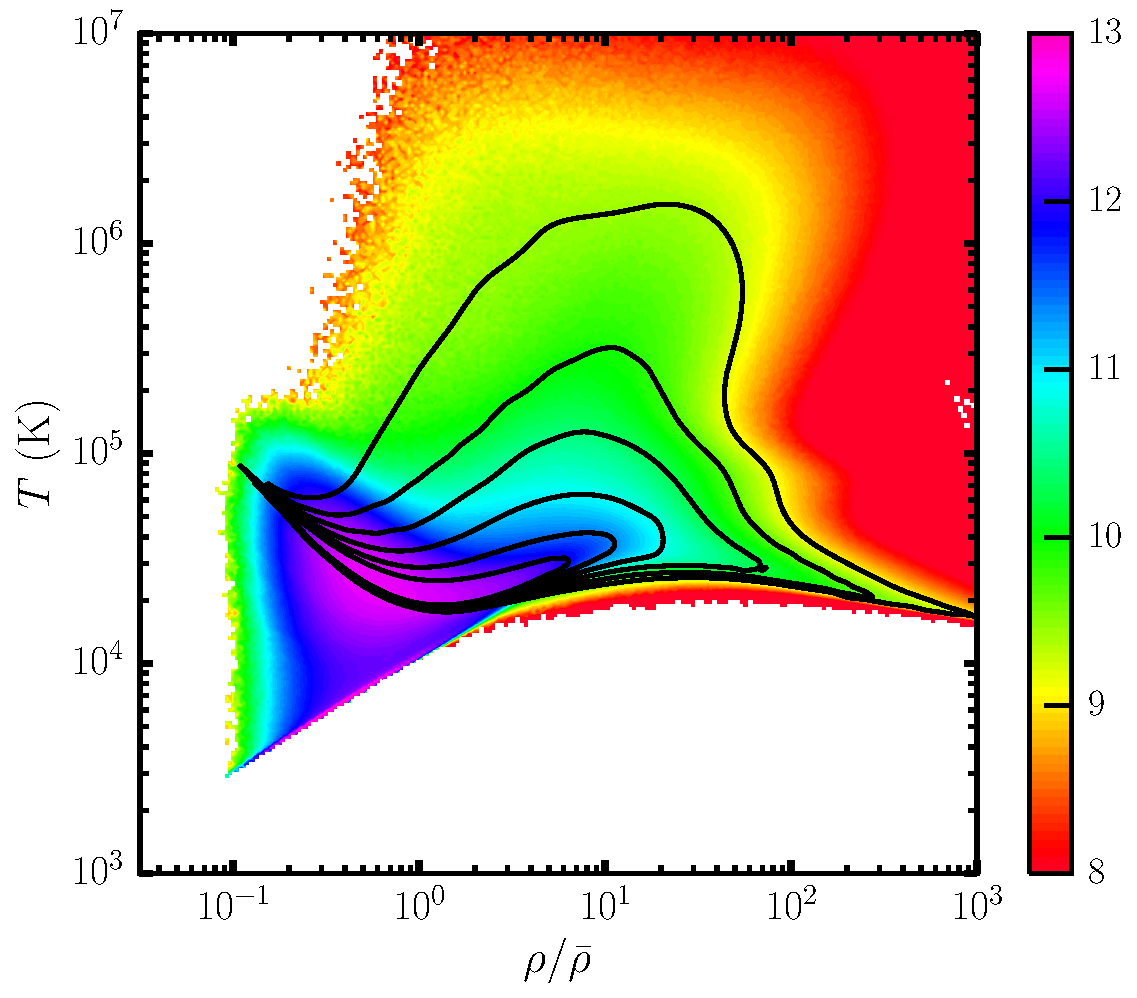
\includegraphics[width = .3\textwidth ]{T_rho_z3_qso.pdf}
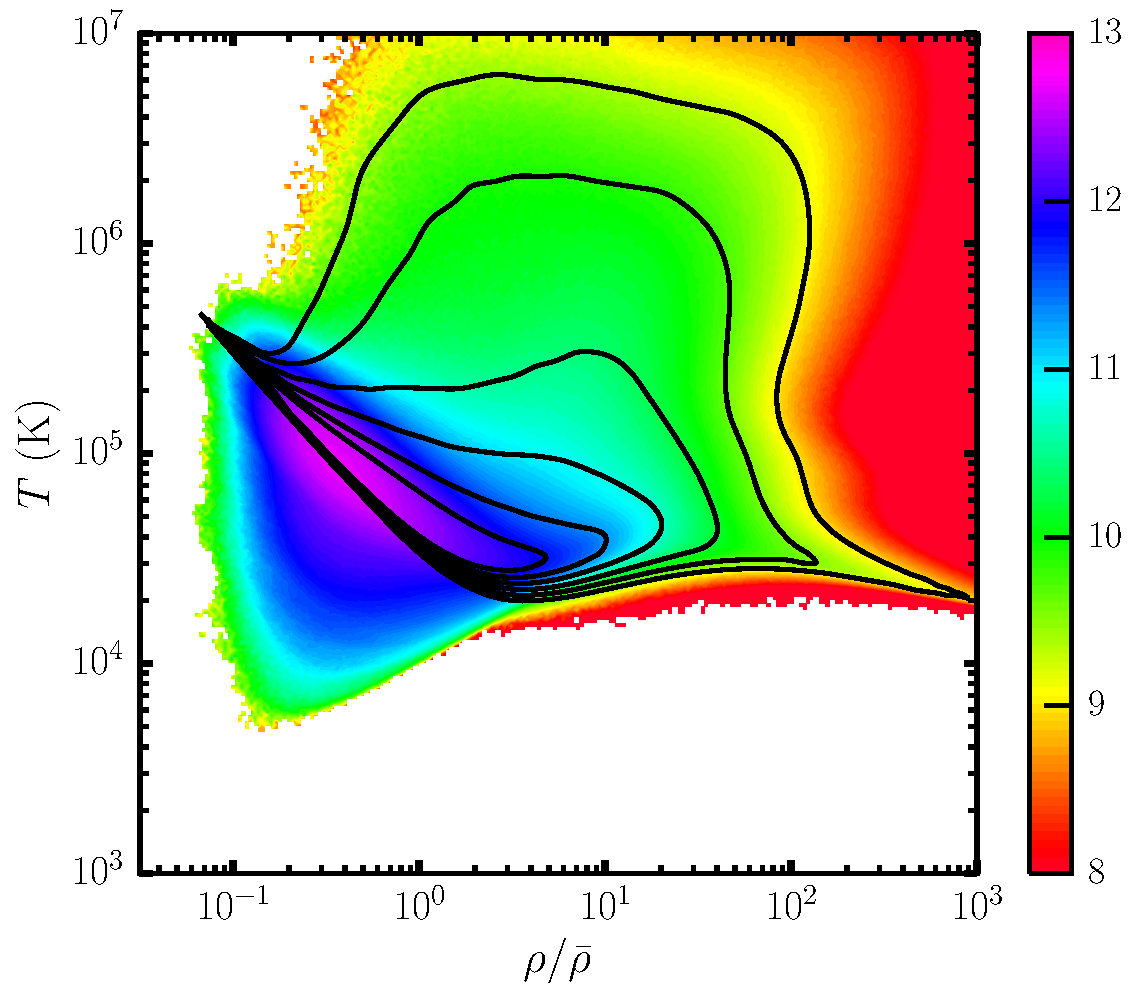
\includegraphics[width = .3\textwidth ]{T_rho_z2_qso.pdf}
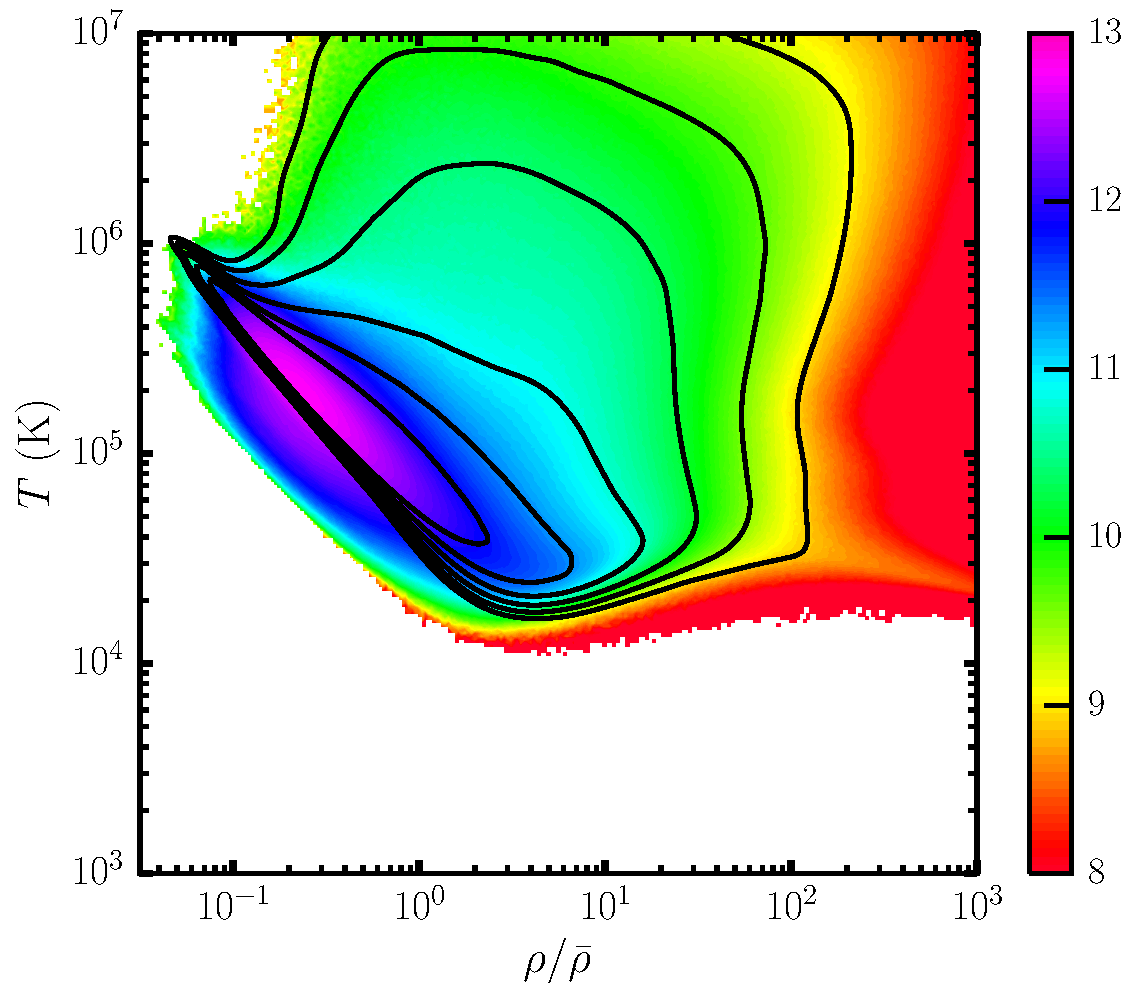
\includegraphics[width = .3\textwidth ]{T_rho_z1_qso.pdf}
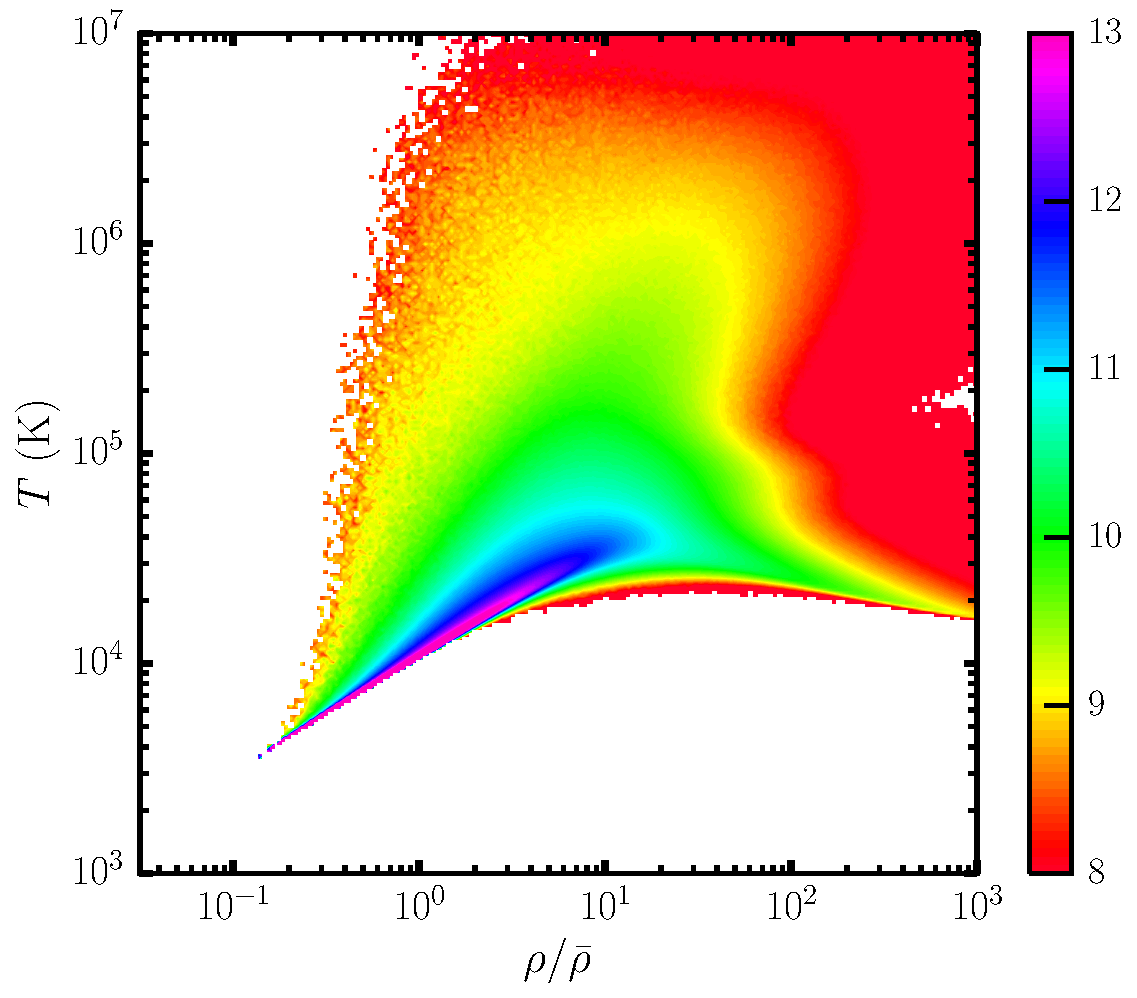
\includegraphics[width = .3 \textwidth ]{T_rho_z3_noheat.pdf}
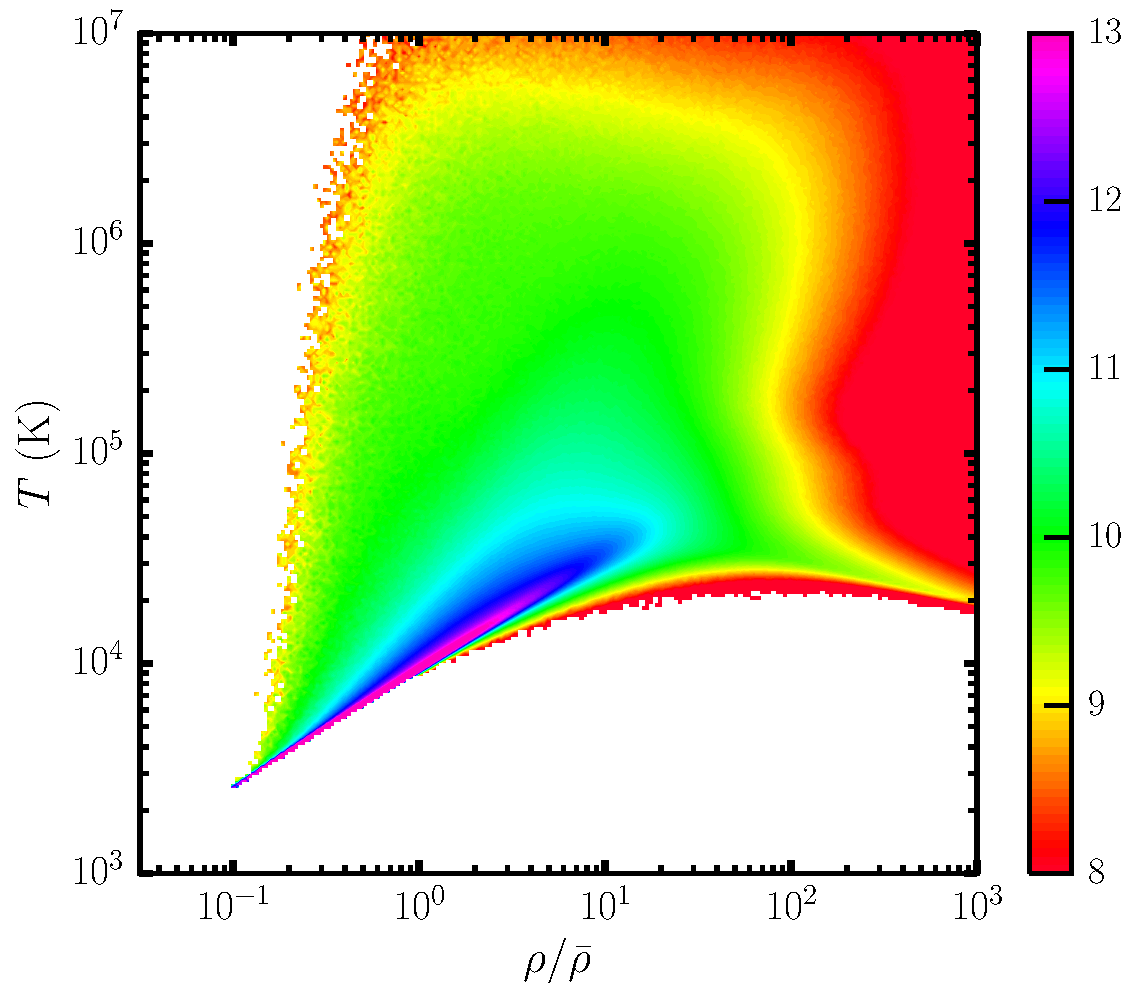
\includegraphics[width = .3\textwidth ]{T_rho_z2_noheat.pdf}
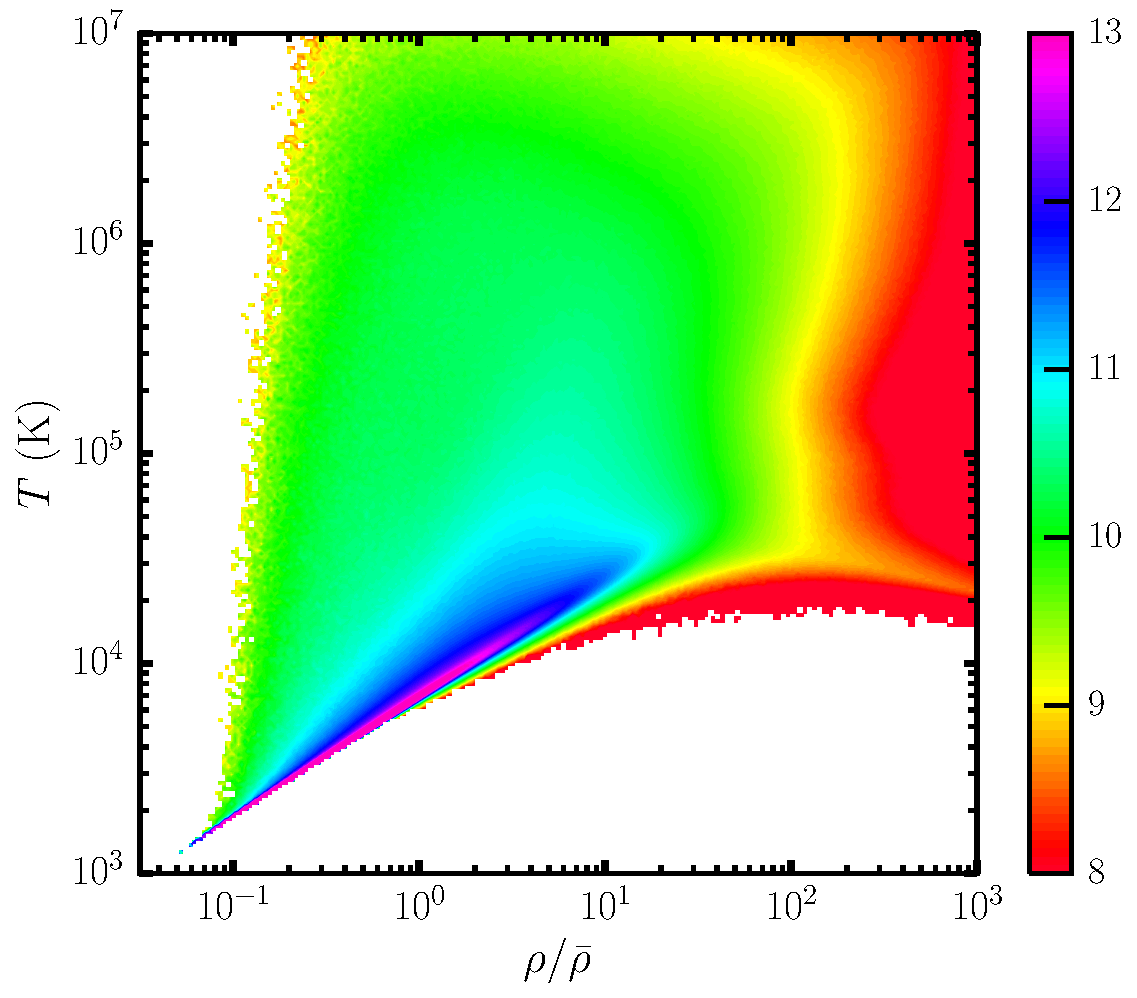
\includegraphics[width = .3\textwidth ]{T_rho_z1_noheat.pdf}
\caption{ Volume-weighted temperature - density relation at $z=3,2$ and 1 (from right to left) for the simulations with no blazar heating (bottom) and inhomogeneous heating (top). The overlying black contours show the corresponding $T-\rho$ relation for uniform blazar heating \citep{2012MNRAS.423..149P} for the same redshift range. The color scale is logarithmic. \ALc{[Add z=0 plot]}}
\label{fig:rho_T}
\end{figure*}

The physical size of the temperature fluctuations in the IGM is mostly set by the mean free path of TeV photons, and is a few tens of Mpc at $z=3$ and increases up to $\simeq$ a Gpc in the present day universe. Fig.~\ref{fig:T_flucs} shows a slice through the midplane of our simulation at $z=3$ for the three heating models we considered. 
\ALc{add slice of T, with typical sizes and discuss. Explain issue of sampling}

\begin{figure*}
\centering
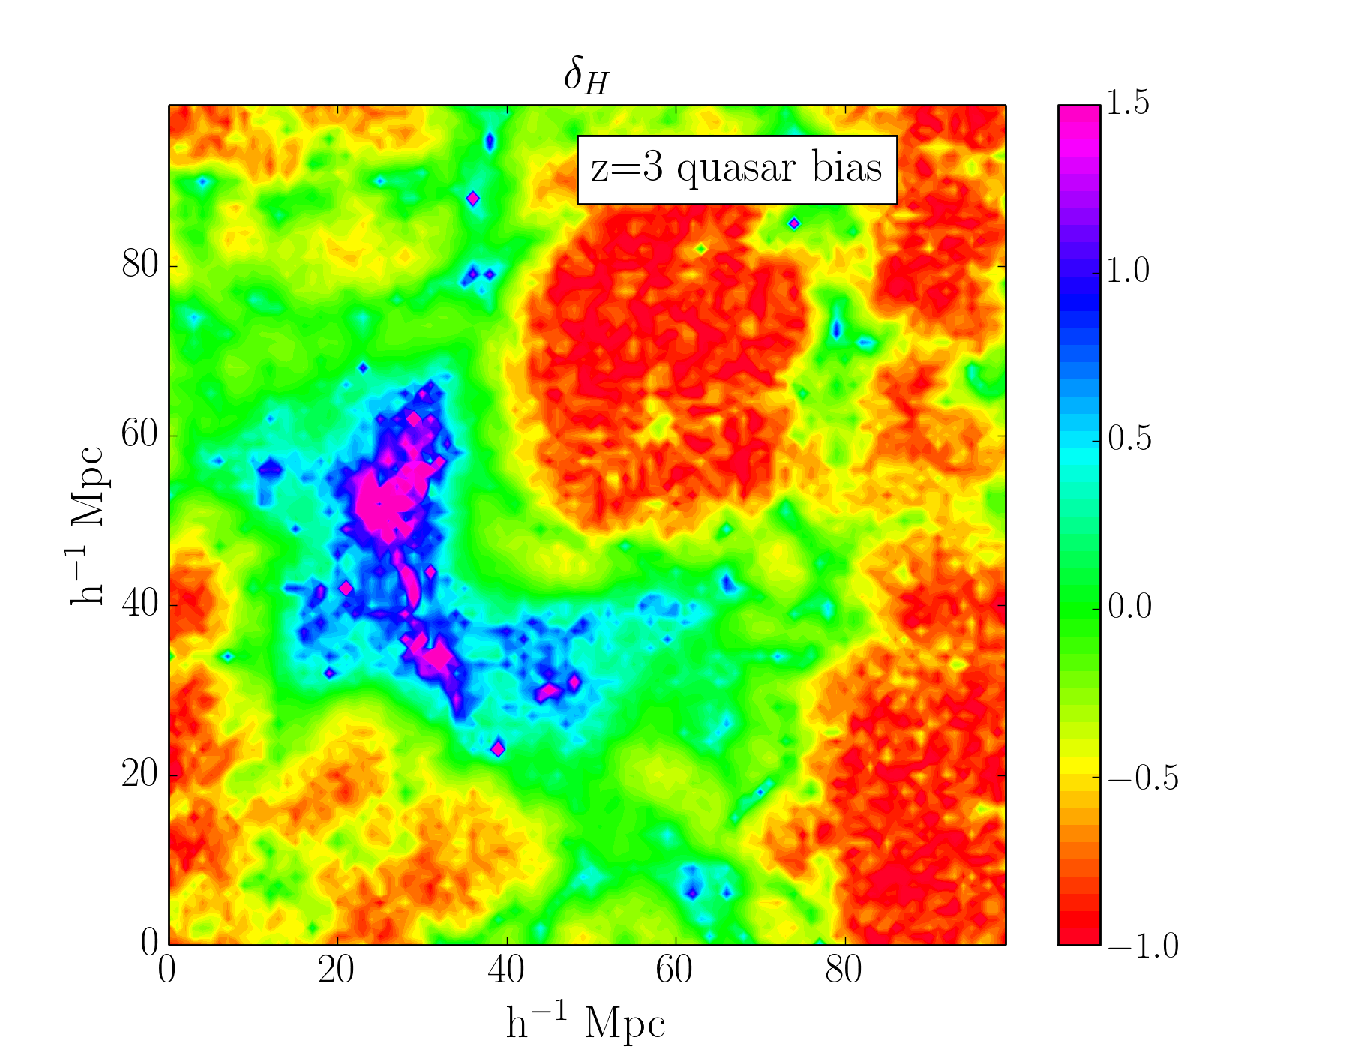
\includegraphics[width = .3\textwidth ]{data_delta_z3_qso4.pdf}
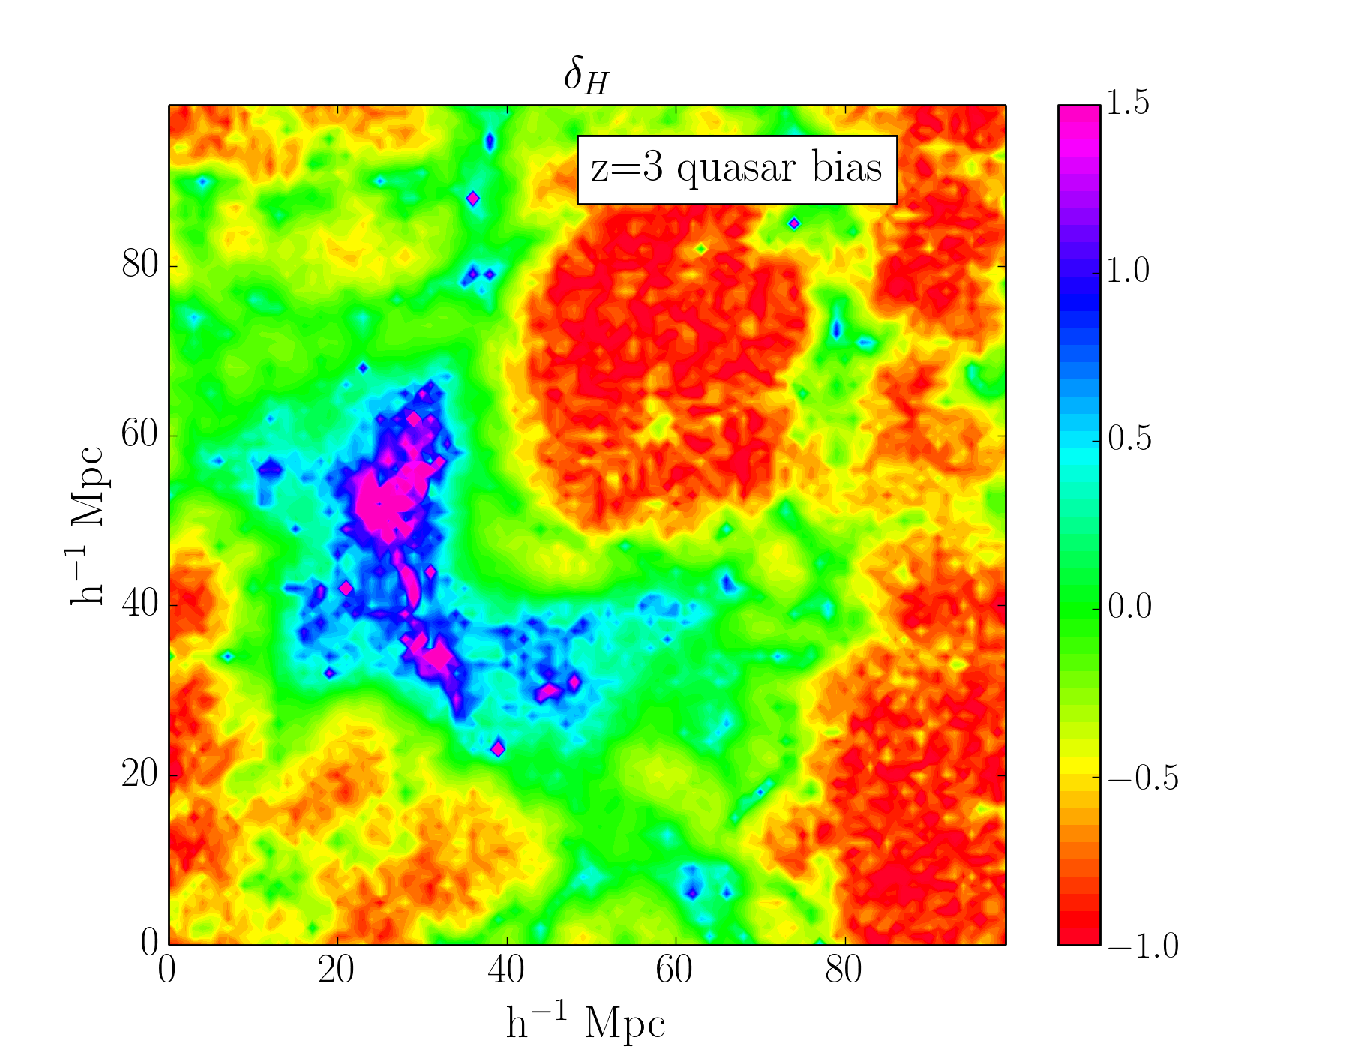
\includegraphics[width = .3\textwidth ]{data_delta_z3_qso4.pdf}
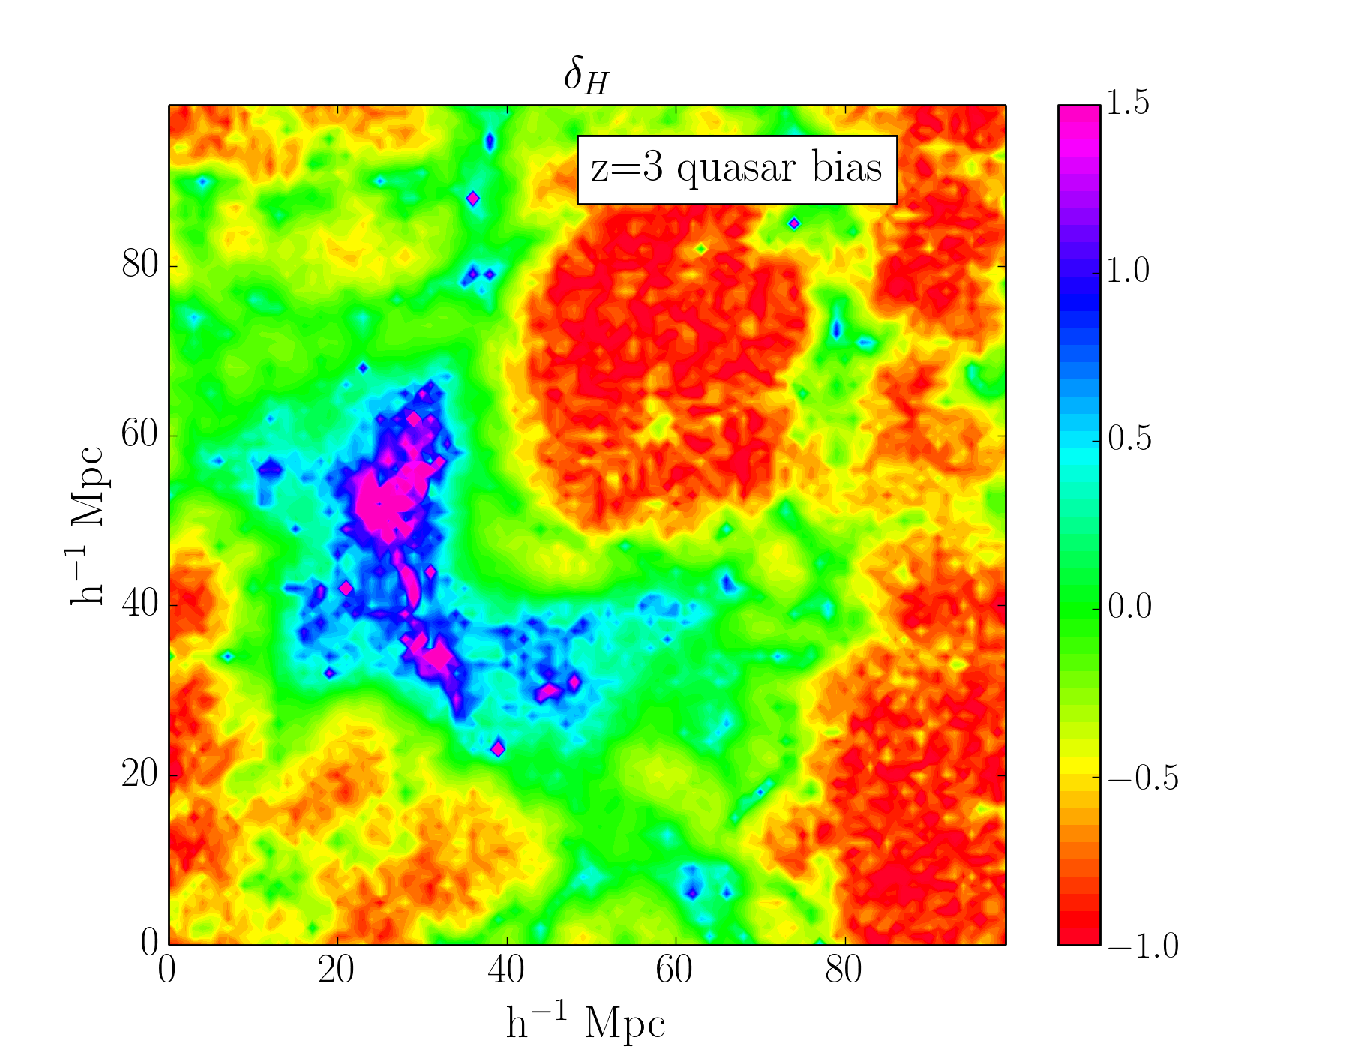
\includegraphics[width = .3\textwidth ]{data_delta_z3_qso4.pdf}
\caption{Distribution of the temperature in the midplane of the simulation domain at $z=2.5$ for the unheated case (left), inhomogeneous heating case (middle) and the uniform heating model (right).\ALc{[Placeholder, plots need to be made]}}
\label{fig:T_flucs}
\end{figure*}


In the next section, we show how the shape of the temperature-density distribution and the size of the temperature fluctuations affect the observable properties of the Ly$\alpha$ forest and compare with the observational data.
%Both the shape of the temperature-density distribution and the physical size of the temperature flucuations are key aspects of blazar heating



% \begin{itemize}
% \item Details about subdividing LOS in chunks for VPFIT
% \end{itemize}

\section{Comparison with observations}\label{sec:obs}
% be explicit about new data?
We compare our simulations with different heating models with observations of the Ly$\alpha$ forest. In this section,  we focus on statistics that are sensitive to low density regions and new observational data. In the Appendix, we provide comparisons with the data and simulations presented in  \citet{2012MNRAS.423..149P} for consistency. 

\subsection{Rescaled flux PDF}
\citet{2017MNRAS.466.2690R} recently proposed a new method to probe the thermal state of the low-density IGM.  In this method the transmitted flux is rescaled by a factor A, which makes it more sensitive to high-transmission regions of the flux PDF, which are likely corresponding to the low-density regions. To compare with the rescaled flux PDF by \citet{2017MNRAS.466.2690R}, we carefully perform the same steps. First, we rescale the optical depth so that the mean transmitted flux $F$ matches the observed value at that redshift \citep{2013MNRAS.436.1023B}. We perform this operation at once for all lines of sight resulting from the same output.  Then, we smooth the flux with a Gaussian of full width at half maximum of $7.2$ km s$^{-1}$ (to model the aperture of the slit) and rebin it into bins of $\Delta v=2.5$ km s$^{-1}$ (resolution of the UVES spectrograph). We then add Gaussian noise with $\sigma=(\sigma_0^2+F(\sigma_c^2-\sigma_0^2))^{1/2}$ with $\sigma_0=0.0028$ and $\sigma_c=0.0088$ (see Appendix F in \citet{2017MNRAS.466.2690R}). To avoid uncertainties due to continuum placement, we then rescale the transmitted flux to the transmitted flux in the 95$^{th}$ percentile. The latter is close to the peak of the flux PDF, and is therefore less noisy than the mean. This operation performed independently for each line of sight, in chunks of size 10 Mpc/h. Finally, to enhance the impact of low density regions, we rescale the optical depth by a factor $A=10$, which yield a rescaled transmitted flux $F_A=F^A$.

%To properly compare the observed spectrum with the simulation, we have to reconstruct a comparable pathlength $dl(z)$ from the simulations.

To reconstruct the pathlength of the Ly$\alpha$ absorbers in the  observed line-of-sight, we stitch together subsections of lines of sight from all outputs between $z=3$ and $z=2.6$. For each output, the size of the subsection is set by the comoving distance $dl$ corresponding to $dz=0.1$ for the considered redshift. The first pixel of the subsection is randomly chosen along one  of the lines of sight and we use the periodic boundary conditions to complete the line of sight if the edge of the computational box is reached before $dl$ is completed. The lines of sight are randomly chosen for each output. While this produces small discontinuities at the junctions of the subsections, it is a more realistic representation of the varying cosmic structure that would be encountered by a photon \citep[see e.g.][for a discussion]{2016arXiv161203935H}. This method implicitly assumes that the removal of contaminants in the observed sightline (such as metals) does not affect the redshift distribution of the Ly$\alpha$ absorbers along the path covered by  the quasar sigtline.

Fig.~\ref{fig:PDF_A} shows the PDF of $F_A$ in our three different heating models, compared with the observed PDF.  As the observed line of sight is unique, cosmic variance can significantly affect the resulting flux PDF \citep{2013MNRAS.428..540R,2017MNRAS.466.2690R}. To provide some measurement of the spread of the flux PDF, we recreate a total of one hundred  lines of sight from each of our simulations (following the method described above). The pink and red regions in Fig.~\ref{fig:PDF_allz_100lines} show the resulting one and two sigma deviations from the mean. While we are confident that we do not oversample specific locations of the simulation, in PaperI we showed that the typical length scale  of heated/unheated regions is of a few tens of Mpc/h. As such, the number of regions sampled by our simulation is somewhat limited and we likely underestimate cosmic variance. 


Fig.~\ref{fig:PDF_A} shows that the rescaled flux PDF of the Lyman $\alpha$ forest cannot be reproduced by a model without additional heating before or around $2.5<z<3$. Inhomogeneous blazar heating does provide a flux PDF compatible with observations. The uniform model, where the same total amount of blazar heating is injected, shows less good agreement with the data. This model has less physical motivation, as blazar heating is naturally inhomogeneous, because of the biased distribution of the sources.  At the redshifts considered, the impact of extended and/or late HeII reionization cannot be ruled out \ALc{[Although it might be more uniform in this case? ]}.  Fig.~\ref{fig:PDF_A1} shows the regular (A=1)  flux PDF in the three heating models, compared with the data from \citet{2013MNRAS.428..540R}. The data shows equally good agreement with all models, meaning that this statistic is not fit to study the properties of the low-density IGM.







\begin{figure*}[h]
\centering
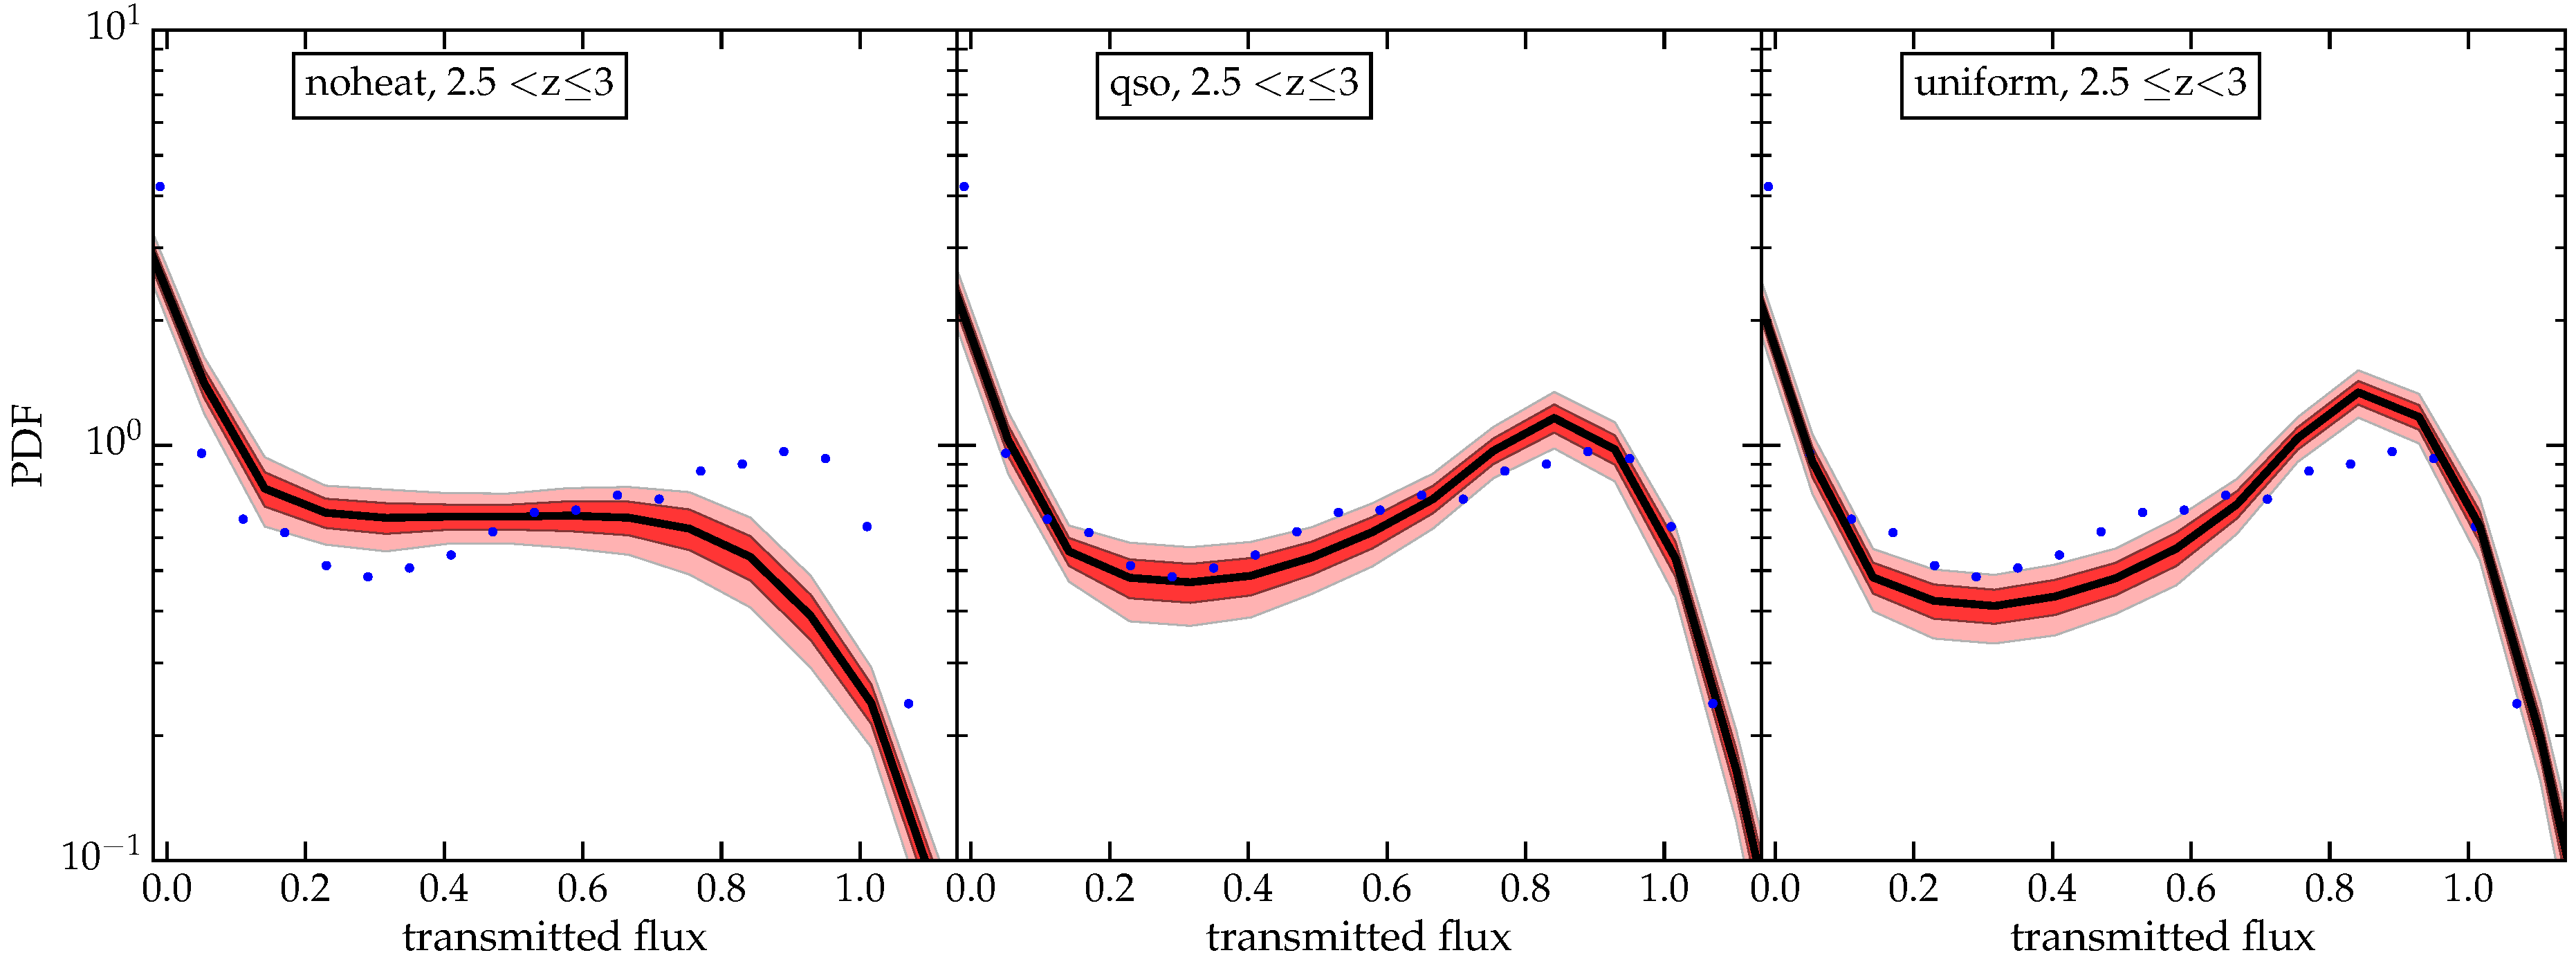
\includegraphics[width = .9\textwidth ]{PDF_allz_100lines}
\caption{Probability distribution function of the rescaled flux in the unheated (left), inhomogeneously heated (middle) and uniformly heated model (right) between $2.5 <z\leq 3$. The thick line represents the mean over the 100 lines of sight, and the red and pink area the 1 and 2 $\sigma$ uncertainty around the mean. The observed PDF is given with the blue dots \citet{2017MNRAS.466.2690R}. }
\label{fig:PDF_A}
\end{figure*}


\subsection{Properties of absorption lines}

The statistical properties of the line-width $b$  and column density $N_{HI}$ of the individual Ly$\alpha$ absorption lines carry information about the density and temperature of the IGM. Schaye determined that it can be used as a proxy for the temperature-density relation in the low-density regime. This is based on the assumption that \ALc{[check column density]}. It also assumes that, for a given column density, the smallest Doppler width is only set by thermal broadening while higher values result from turbulent motions within the absorbers. Intrinsically, this method assumes a unique relation between temperature and density, whereas the inhomogeneous blazar heating model shows a wide distribution (see Fig. \ref{fig:T-rho}. 

We compare our simulations with the data from \citet{2012ApJ...757L..30R}, based on 15 quasar absorption lines, as part of the Keck Baryonic Structure Survey (KBSS \ALc{cite Steidel, Rudie papers]}. The sample covers a total pathlength $dz=8.27$ between $2.02\leq z \leq 2.84$ with a mean redshift $\bar{z}=2.34$. The data was obtained with the HIRES spectrograph, with a FWHM$\simeq 7$ km s$^{-1}$ and typical S/N 50-200.  We specifically focus on the low column density $log(N_{HI} \leq 14)$, corresponding to low density optically thin absorbers. Those are the most likely not associated with galaxies, but with the IGM \ALc{[cite]}. 

In order to determine the line widths and column density of the absorbers, each of them has to identified and individually fit. \citet{2012ApJ...757L..30R} use the VPFIT software \ALc{[add link here]}, which automatically finds the properties ($z,b,N_{HI}$) of the absorbers using a $\chi^2$-reducing method. Lines with $b \leq 8$ or $b \geq 100$ or relative errors larger than 50$\%$ for the properties of the absorbers are discarded from the initial sample. 

To enable the closest possible comparison, we also use VPFIT to analyse our 100 lines of sight. Especially at the highest redshifts, each line of sight contains too many absorbers ($\gtrsim 150$) that the converges of VPFIT is really slow. As such, we divide each line of sight into 5 equally-sized chunks and analyse each of them separately. At the end, we concatenate the absorbers from the 5 sections into one list. We remove the absorbers within $dv=500$ km s$^{-1}$ of the edges. Visual inspection determined that this is a satisfactory way to eliminate boundary effects while maintaining most of the sample. We have tested cuts up to 1000 km s${-1}$ and find no difference in the following results. Then, we perform the same additional cuts than \citet{2012ApJ...757L..30R}. Finally, properly combining randomly selected absorbers from our different outputs, we select a subsample of absorbers with the same pathlength distribution $dl(z)$ using the data from Fig.~1 in \ALc{[cite]}. 

Thanks to the  large sample size, we can consider the complete 2D properties of the  absorbers, rather than limiting ourselves to their 1D projections. Although the complete $b-N_{HI}$ distribution carries information on the physical properties of the IGM, oftentimes only the lower enveloppe of the distribution is considered \ALc{[cite]}. The \citet{2012ApJ...757L..30R} sample increases the number of well-characterised Ly$\alpha$ absorbers in that redshift range by a factor of 10. e


In Fig.~\ref{fig:b_Nh} we show the $b-N_{Hi}$ distribution in the uniform (top left), inhomogeneous (top right) and unheated model (bottom left) compared with the data (bottom right). From these plots it is clear that the complete 2D distribution is different in the three heating models and that one should not restrict the distribution. As such, the broad temperature-density distribution in the inhomogeneous heating case imprints the $b-N_{HI}$ distribution, which is an intermediate case between the unheated and the uniformly heated case. 

By eye, the R12 sample looks closest to the unheated model. Although the inhomogeneous heating model successfully reproduces the lower enveloppe of the R12 distribution,  the peak of both distributions are offset. \ALc{[quantify]}. The inhomogeneous blazar heating models favors lines with slightly higher values for both the column density and the Doppler width. Fig.~\ref{fig:b_Nh_1d} shows the 1D histograms of the column density and Doppler with and  provides a more quantitative comparison of the models and data. The mode of the Doppler width distribution is higher by $\simeq$ 8 km s$^{-1}$ in 


%The line-width and column density determination requieres a
\begin{figure*}[h]
\centering
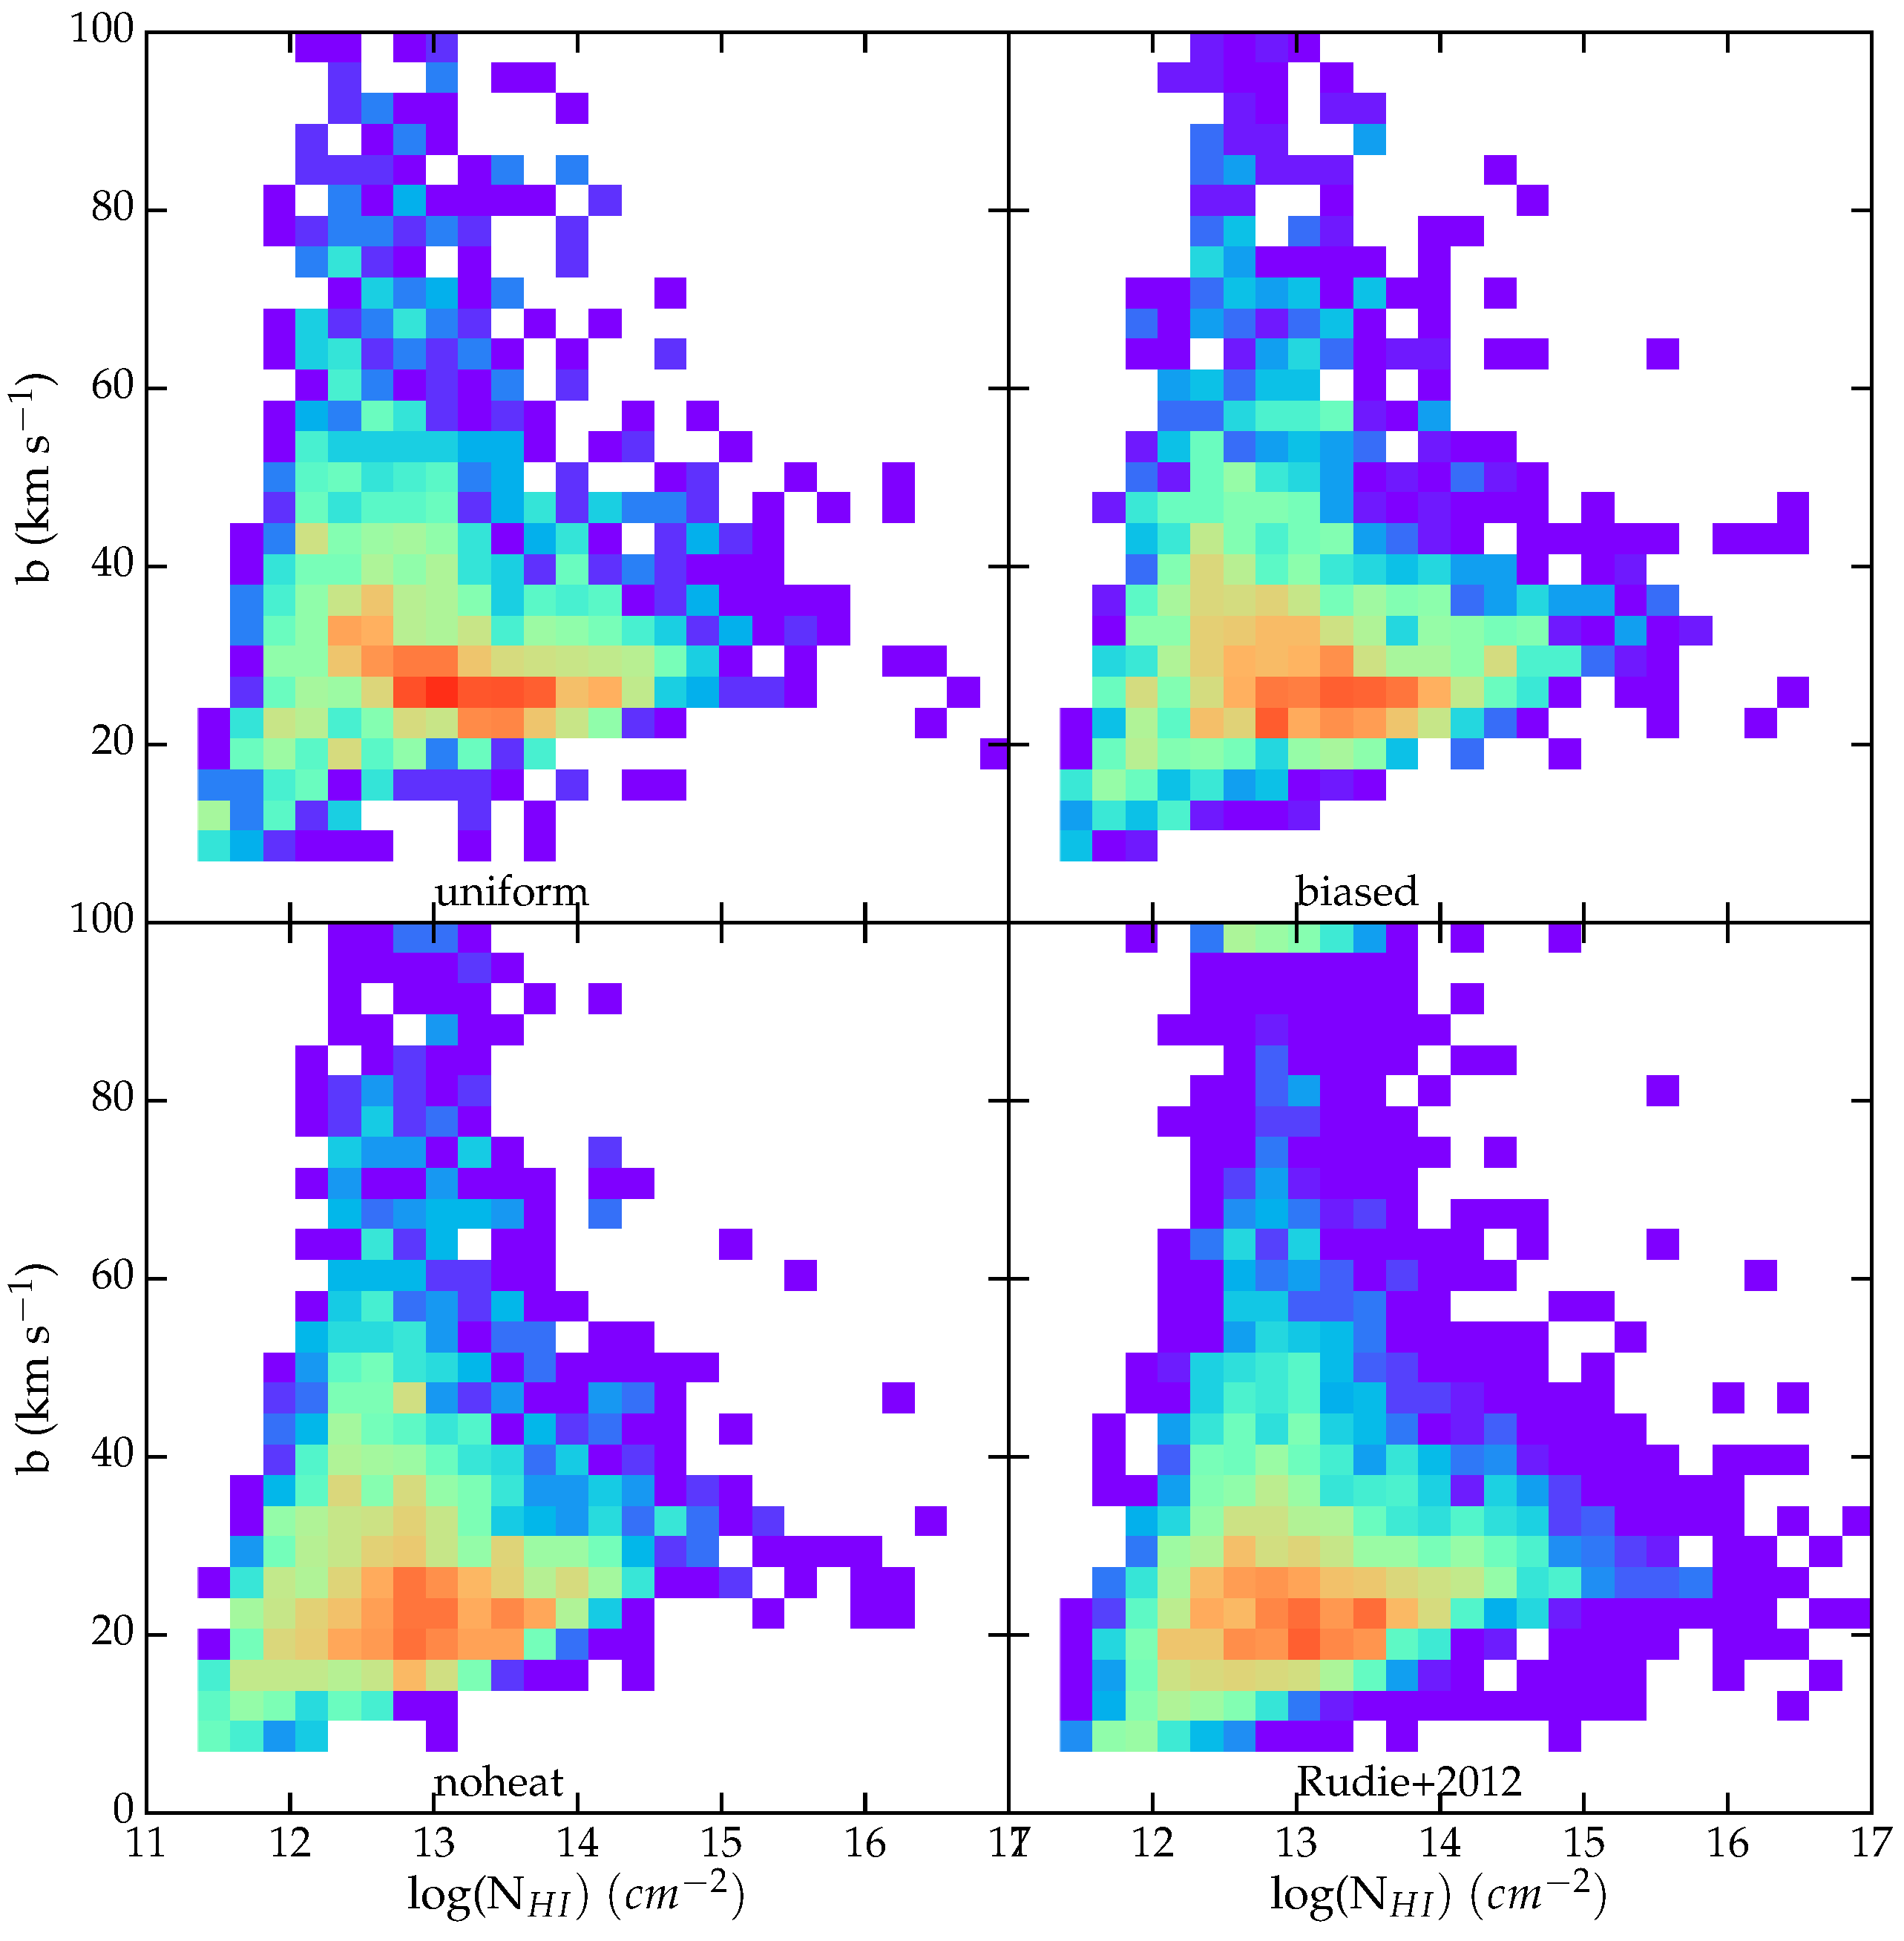
\includegraphics[width = .8\textwidth ]{compare_rudie_bNh.pdf}
\caption{Line-width versus $HI$ column density distribution in the three different heating models, compared with the data from \citet{2012ApJ...757L..30R}.\ALc{[add colorbar, make nicer plot]}}
\label{fig:b_Nh}
\end{figure*}

\begin{figure*}[h]
\centering
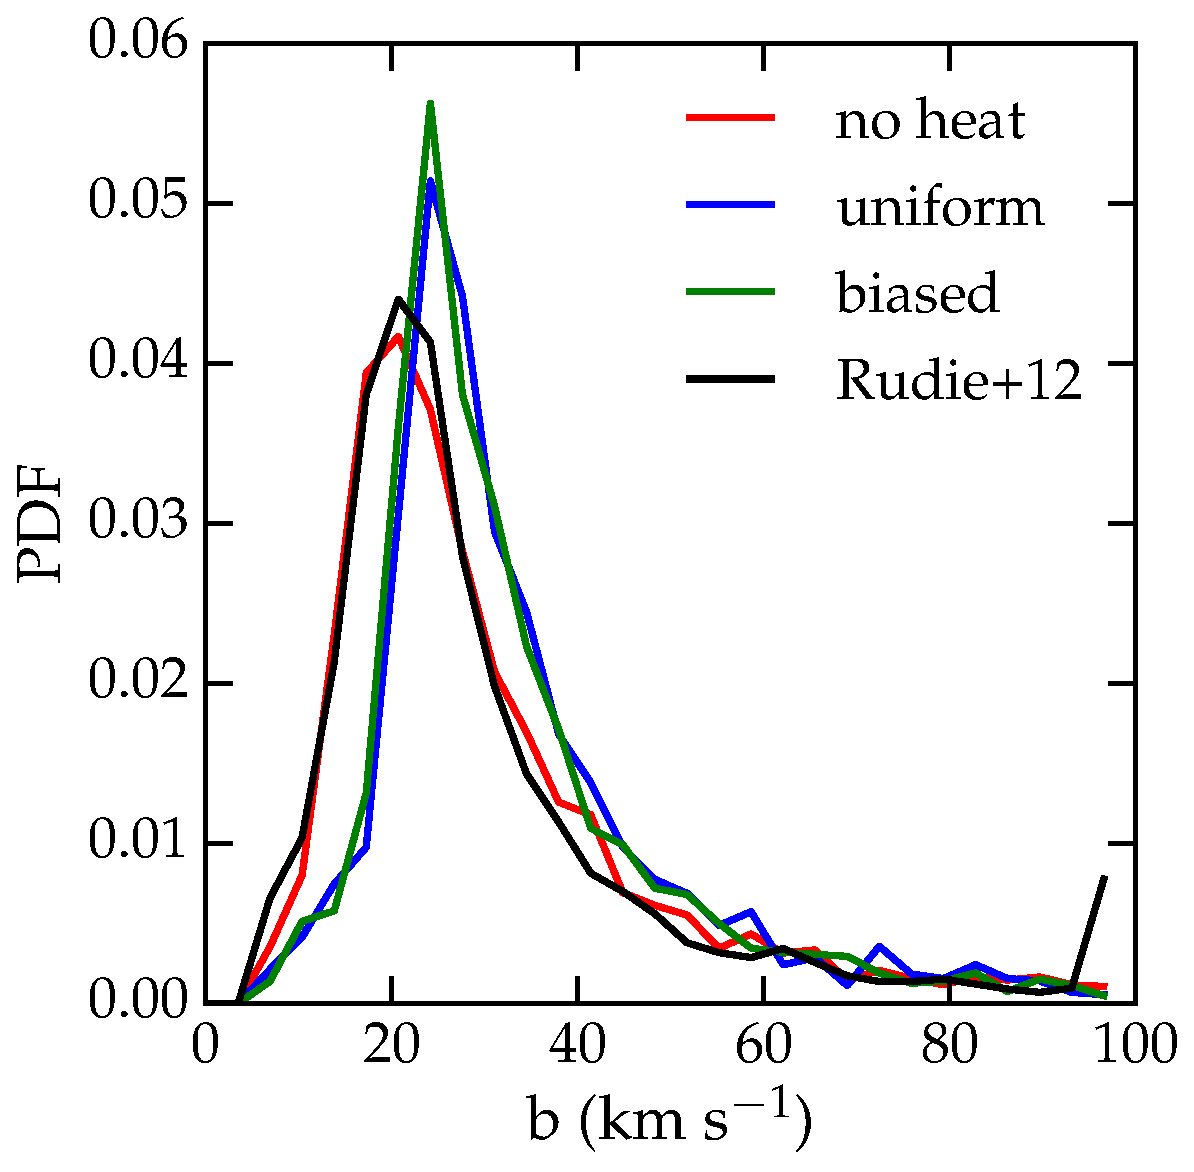
\includegraphics[width = .35\textwidth ]{hist_b_rudie_vs_sims.pdf}
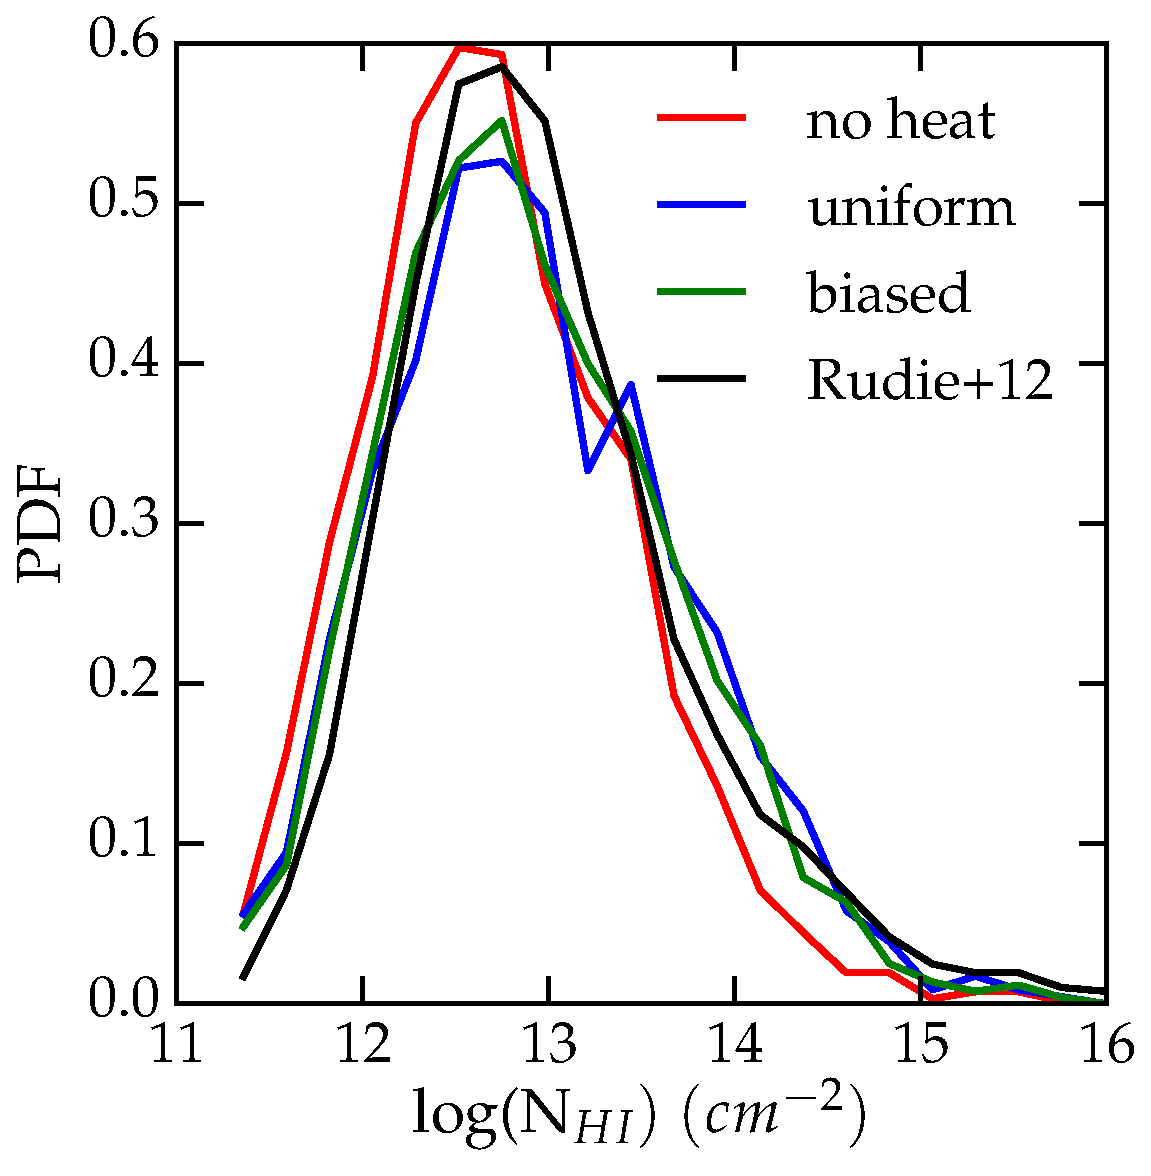
\includegraphics[width = .35\textwidth ]{hist_Nh_rudie_vs_sims.pdf}
\caption{ Line-width (left) and $HI$ column density (right) histograms  in the three different heating models, compared with the data from \citet{2012ApJ...757L..30R}.\ALc{ make nicer plots, add Kim data and error bars. check normalization]}}
\label{fig:b_Nh_1d}
\end{figure*}




\subsection{Low-redshift absorbers}
\ALc{[Do the science! yay!]}

\section{Discussion}\label{sec:discussion}

\begin{itemize}
\item full b nh distribution vs restricted comparisons
\item late He II reionisation?
\item advocate for more data
\end{itemize}
\Ec{We have demonstrated above that accounting for a heating of the low-density IGM by TeV blazars significantly improves the agreement between the observed PDF of the rescaled flux and theoretical predictions. The same additional heating allows to better match the observed widths of Lyman-$\alpha$ absorption lines at redshifts ???. These findings are consistent with \citep{} but ... . To interpret these findings it is important to understand whether blazar heating is the only plausible effect that can bridge these gaps or whether there are other effects, such as alternative heating mechanisms, that can potentially ease these tensions. In particular HeII reionization is expected to provide significant heating to the IGM. The redshift range over which this happens is somewhat uncertain. Measurements of the transmitted flux in the HeII Lyman-$\alpha$ show little scatter below redshift $2.7$ \citep{2016ApJ...825..144W} suggesting that a patchy HeII reionization is largely over at this point and that most of the heating should have happend before that. }

The impact of HeII reionization on the temperature of the IGM cannot be ruled out for $z>2.5$. As such, a clear signature of a heating source in low density IGM, for which blazar heating is currently the only candidate, can only be firmly established with lower redshift measurements. While $z<2.5$ data is present in the DEEP spectrum, the data contains both Ly$\alpha$ and Ly$\beta$ absorption lines, which makes the analysis more complex and prone to uncertainties, especially when the sample is limited. Figure ~\ref{fig:PDF_predict} shows the predicted PDF of the rescaled flux between $2.5<z<2$ for the three models we consider. High signal-to-noise, high spectral resolution lines-of-sight towards quasars located between $2.2\lesssim z \lesssim 2,7$ (not contaminated by Ly$\beta$ absorption) will be able to discriminate between a heated and non-heated model. 
 %At lower redshifts, 




\begin{figure*}[h]
\centering
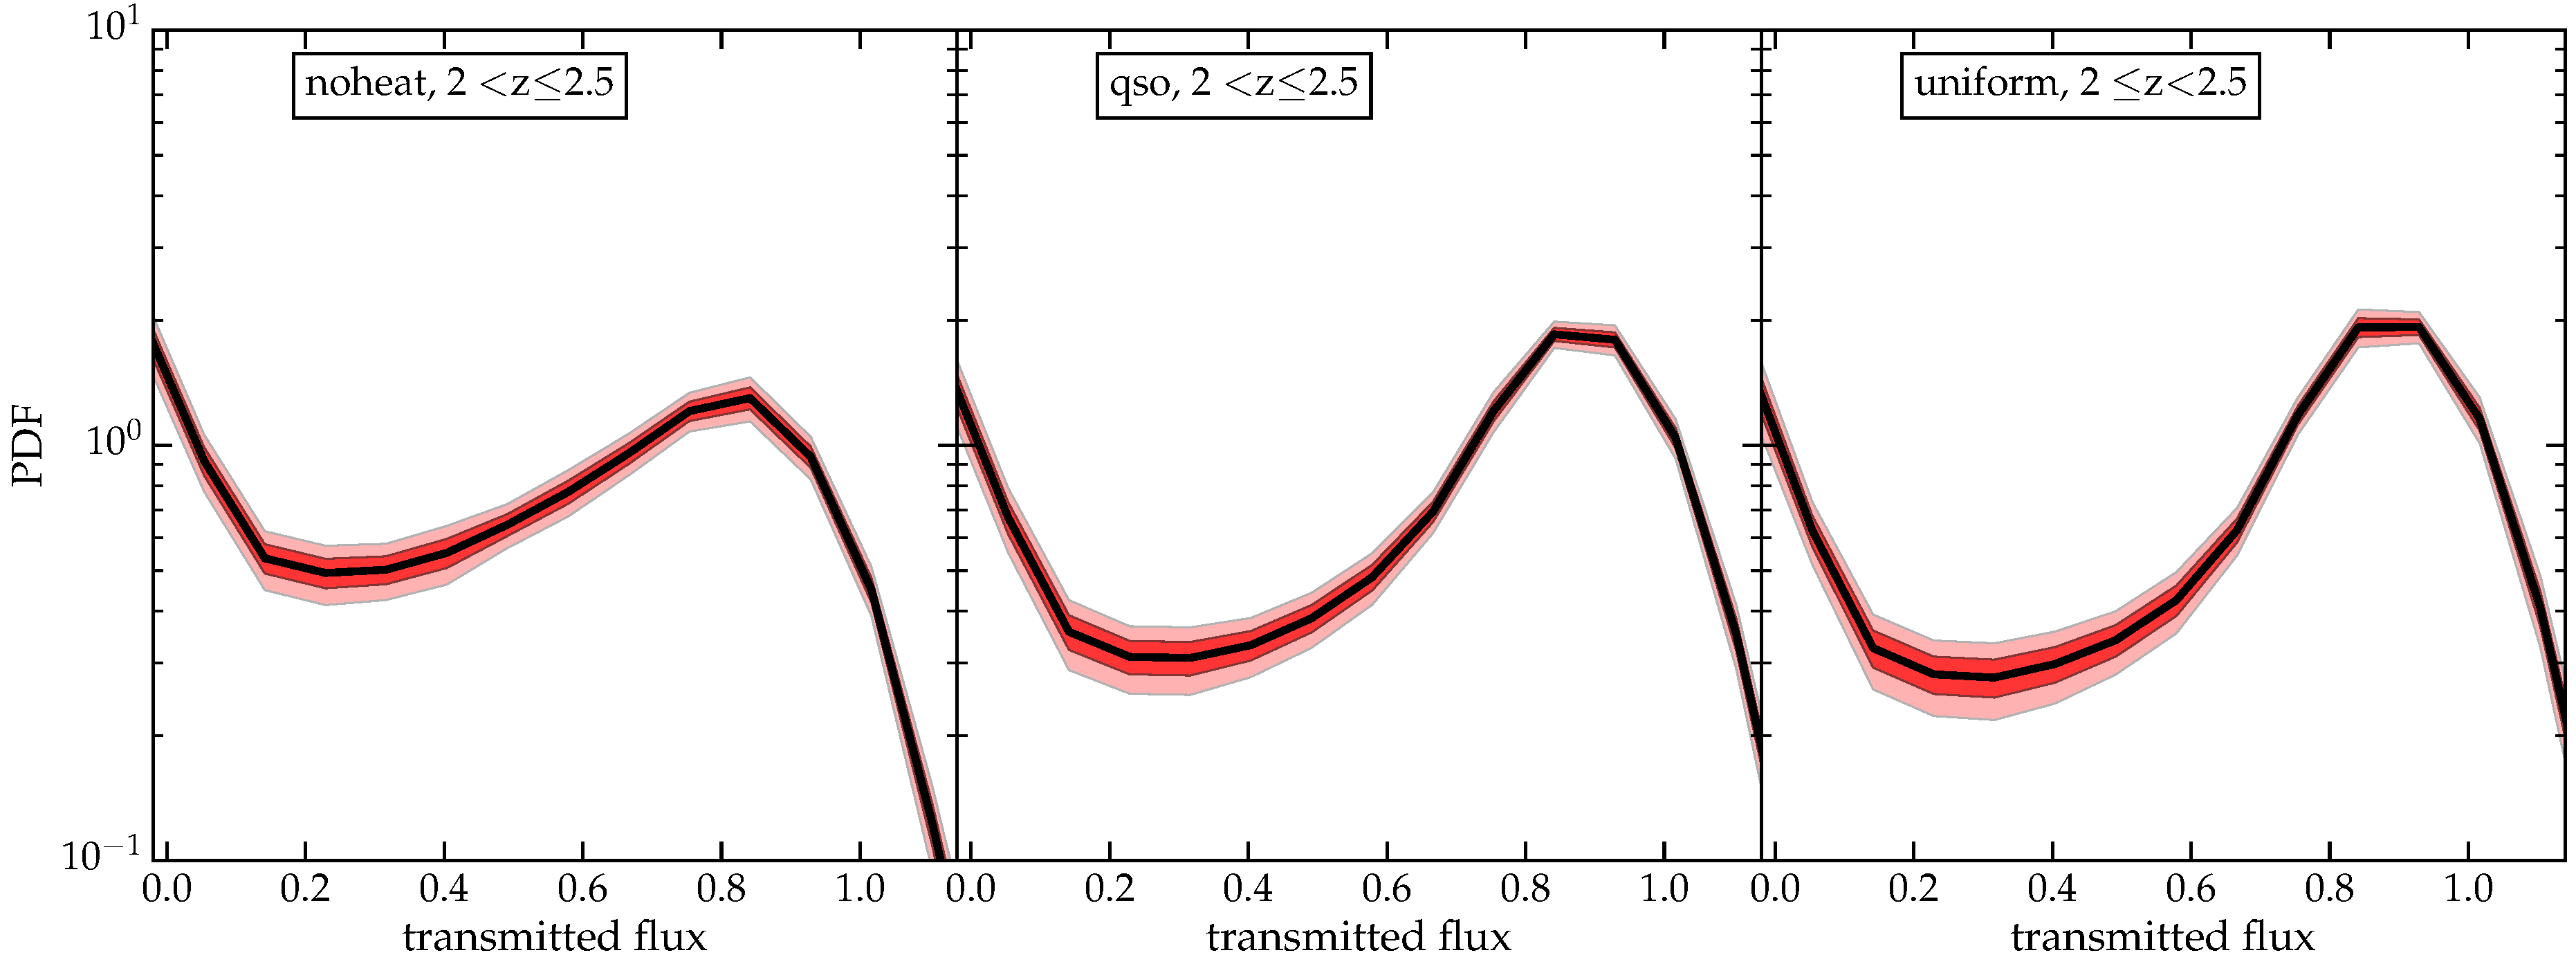
\includegraphics[width = .9\textwidth ]{PDF_predict_allz_100lines}
\caption{Predicted probability distribution function of the rescaled flux in the unheated (left), inhomogeneously heated (middle) and uniformly heated model (right) between $2 <z\leq 2.5$. The thick line represents the mean over the 100 lines of sight, and the red and pink area the 1 and 2 $\sigma$ uncertainty around the mean.  }
\label{fig:PDF_predict}
\end{figure*}

%\subsection{Predictions}

\section{Conclusions}\label{sec:conclusion}
\appendix
\section{Consistency checks}
% \begin{figure*}[h]
% \centering
% 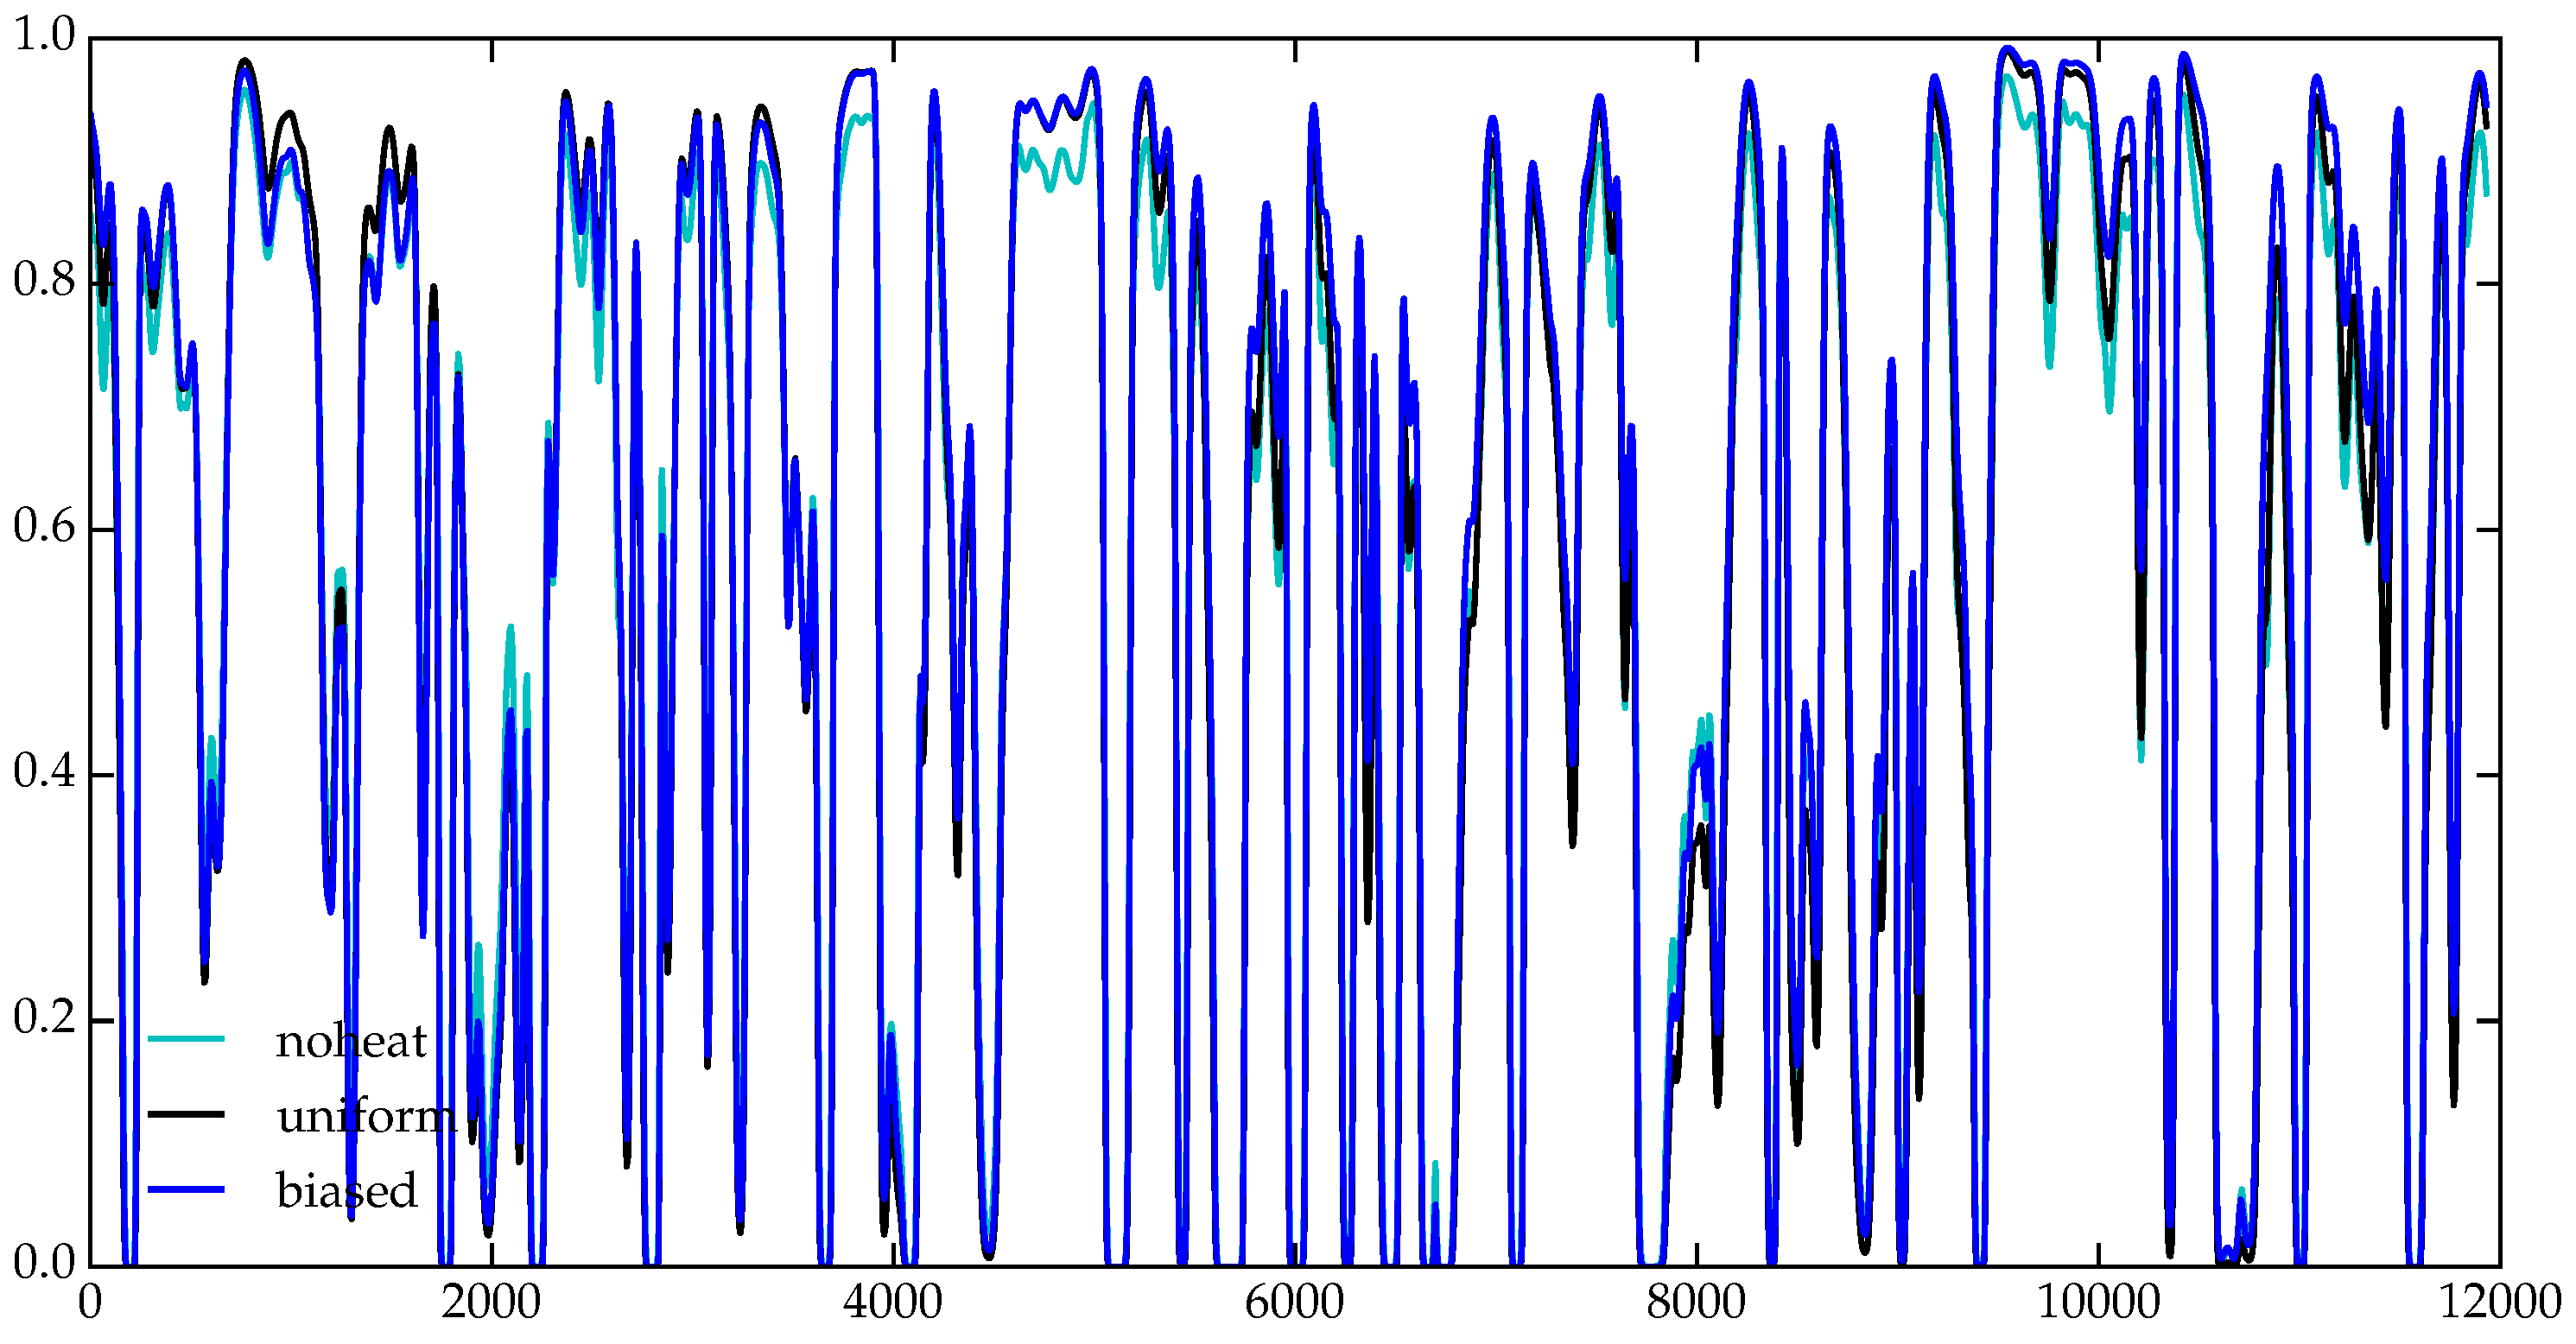
\includegraphics[width = .8\textwidth ]{lines_z2_2}
% \caption{Ly$\alpha$ absorption spectrum at $z=2.2$ in the three models. \ALc{[Placeholder, will be improved]}}
% \label{fig:bias}
% \end{figure*}

\begin{figure}[h]
\centering
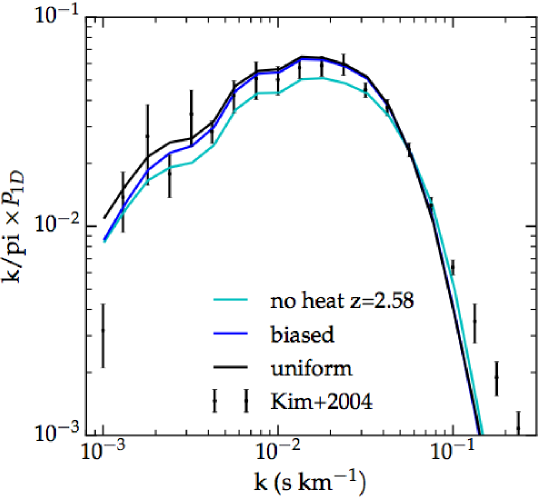
\includegraphics[width = .45\textwidth ]{powerspec}
\caption{ Power spectrum at different redshifts compare with observations \ALc{[Placeholder, will be improved]}}
\label{fig:powespec}
\end{figure}

\begin{figure}[h]
\centering
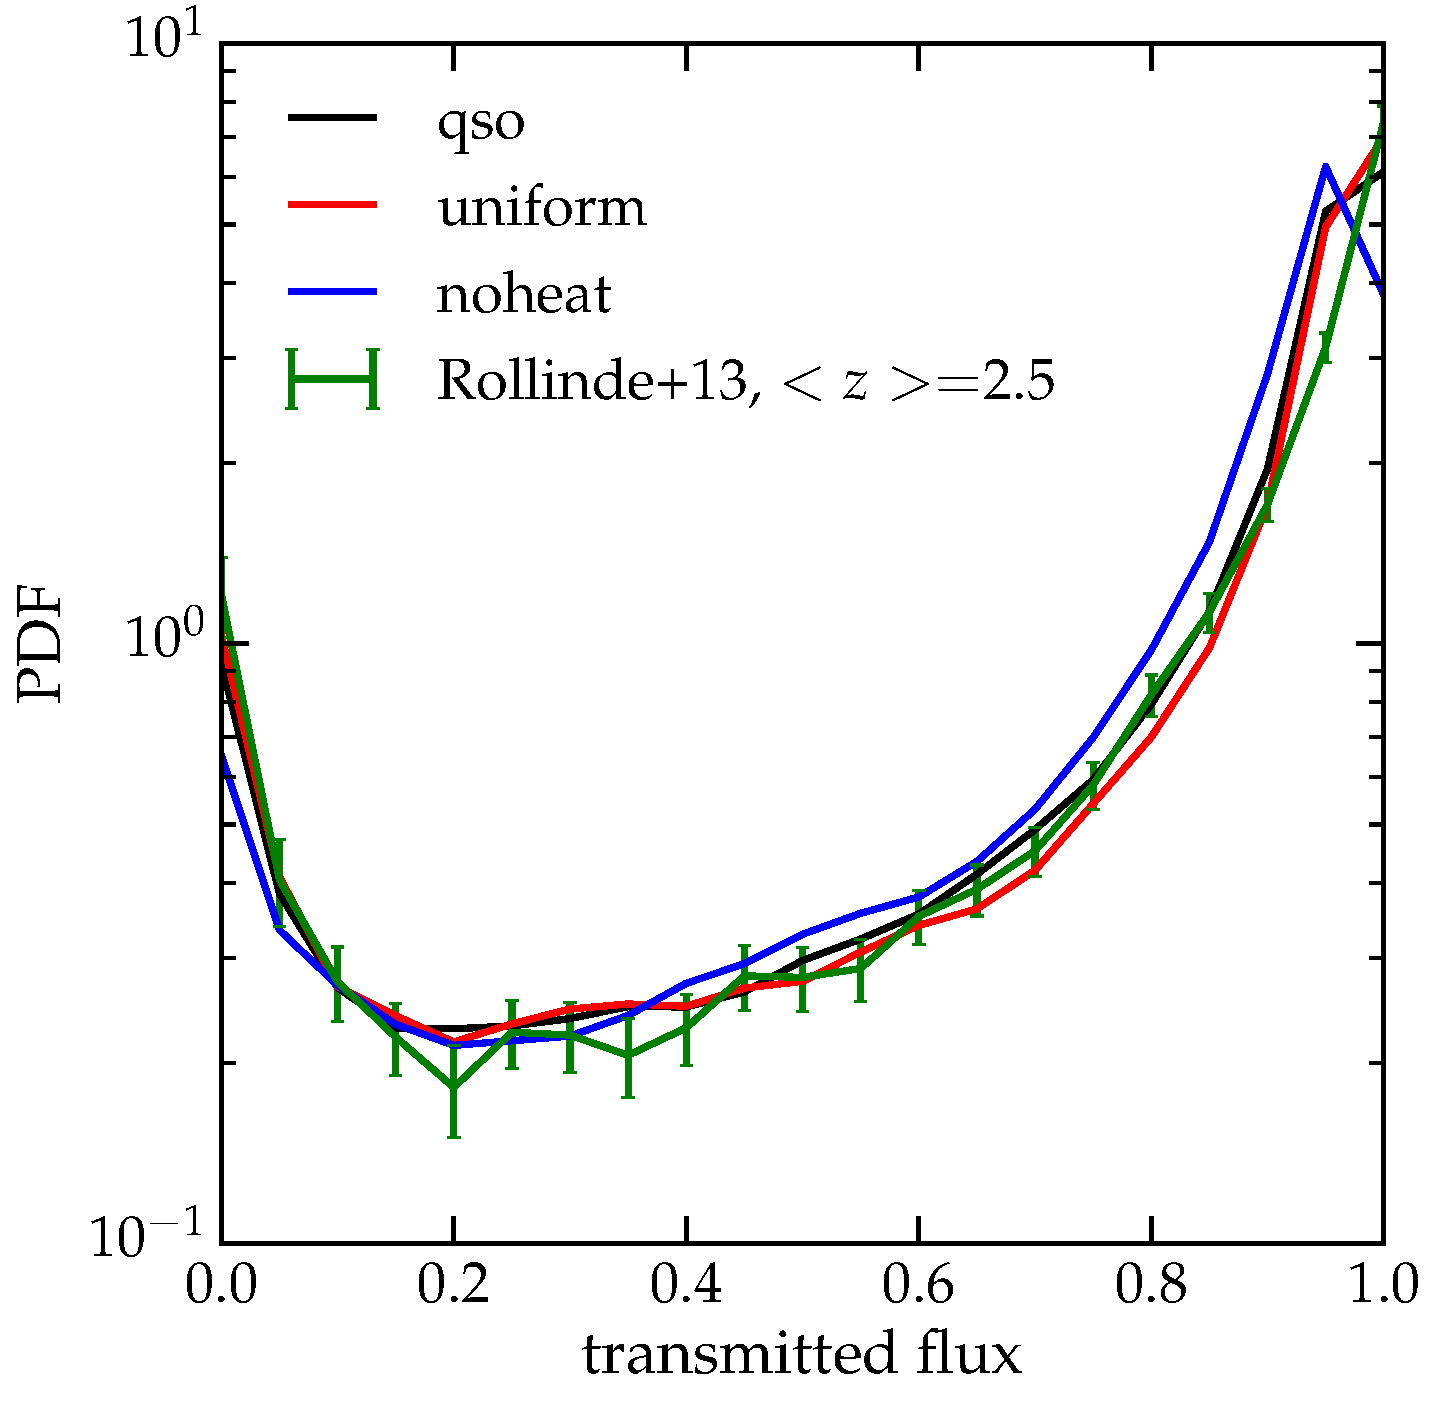
\includegraphics[width = .9\textwidth ]{flux_PDF_Rollinde_25.pdf}
\caption{Reuglar (A=1) flux PDF }
\label{fig:fluxPDF}
\end{figure}

\begin{acknowledgements}
%A.L. warmly thanks Alberto Rorai for sharing an early version of his manuscript and the many clarifications he provided.
%% AL and PC are supported by the UWM Research Growth Initiative, the NASA ATP
%% program through NASA grant NNX13AH43G, and NSF grant AST-1255469.
%% A.E.B.~and M.S.~receive financial support from the Perimeter
%% Institute for Theoretical Physics and the Natural Sciences and
%% Engineering Research Council of Canada through a Discovery Grant.
%% Research at Perimeter Institute is supported by the Government of
%% Canada through Industry Canada and by the Province of Ontario through
%% the Ministry of Research and Innovation.
%% C.P.~gratefully acknowledges
%% financial support of the Klaus Tschira Foundation. E.P. acknowledges support by the ERC grant ``The Emergence of Structure during the epoch of Reionization''.
%% The authors acknowledge the Texas Advanced Computing Center (TACC) at The University of Texas at Austin and the NASA Advanced Supercomputing Division for providing HPC resources that have contributed to the research results reported within this paper. The authors thank S. Furlanetto, A. Loeb and M. Heahnelt for fruitful discussions. 
\end{acknowledgements}


\bibliographystyle{apj}
\bibliography{biblio_total}
\end{document}
